% Options for packages loaded elsewhere
\PassOptionsToPackage{unicode}{hyperref}
\PassOptionsToPackage{hyphens}{url}
%
\documentclass[
  10pt,
]{article}
\usepackage{lmodern}
\usepackage{amssymb,amsmath}
\usepackage{ifxetex,ifluatex}
\ifnum 0\ifxetex 1\fi\ifluatex 1\fi=0 % if pdftex
  \usepackage[T1]{fontenc}
  \usepackage[utf8]{inputenc}
  \usepackage{textcomp} % provide euro and other symbols
\else % if luatex or xetex
  \usepackage{unicode-math}
  \defaultfontfeatures{Scale=MatchLowercase}
  \defaultfontfeatures[\rmfamily]{Ligatures=TeX,Scale=1}
\fi
% Use upquote if available, for straight quotes in verbatim environments
\IfFileExists{upquote.sty}{\usepackage{upquote}}{}
\IfFileExists{microtype.sty}{% use microtype if available
  \usepackage[]{microtype}
  \UseMicrotypeSet[protrusion]{basicmath} % disable protrusion for tt fonts
}{}
\makeatletter
\@ifundefined{KOMAClassName}{% if non-KOMA class
  \IfFileExists{parskip.sty}{%
    \usepackage{parskip}
  }{% else
    \setlength{\parindent}{0pt}
    \setlength{\parskip}{6pt plus 2pt minus 1pt}}
}{% if KOMA class
  \KOMAoptions{parskip=half}}
\makeatother
\usepackage{xcolor}
\IfFileExists{xurl.sty}{\usepackage{xurl}}{} % add URL line breaks if available
\IfFileExists{bookmark.sty}{\usepackage{bookmark}}{\usepackage{hyperref}}
\hypersetup{
  pdftitle={Can galaxy dynamics be explained by real non-baryonic mass and Newtonian gravity? Possibly: a mass that responds to the gravitational potential and enters the Poisson equation only through its source term},
  pdfauthor={James R. Marsen},
  hidelinks,
  pdfcreator={LaTeX via pandoc}}
\urlstyle{same} % disable monospaced font for URLs
\usepackage[margin=2.2cm]{geometry}
\usepackage{graphicx}
\usepackage{longtable,booktabs,array,calc}
\makeatletter
\def\maxwidth{\ifdim\Gin@nat@width>\linewidth\linewidth\else\Gin@nat@width\fi}
\def\maxheight{\ifdim\Gin@nat@height>\textheight\textheight\else\Gin@nat@height\fi}
\makeatother
% Scale images if necessary, so that they will not overflow the page
% margins by default, and it is still possible to overwrite the defaults
% using explicit options in \includegraphics[width, height, ...]{}
\setkeys{Gin}{width=\maxwidth,height=\maxheight,keepaspectratio}
% Set default figure placement to htbp
\makeatletter
\def\fps@figure{htbp}
\makeatother
\setlength{\emergencystretch}{3em} % prevent overfull lines
\providecommand{\tightlist}{%
  \setlength{\itemsep}{0pt}\setlength{\parskip}{0pt}}
\setcounter{secnumdepth}{-\maxdimen} % remove section numbering

\title{Can galaxy dynamics be explained by real non-baryonic mass and Newtonian gravity?\\[0.6ex]{\large Possibly: a mass that responds to the gravitational potential and enters the Poisson equation only through its source term}}
\author{James R. Marsen\\[2pt]
  {\normalsize Independent researcher, New Jersey, USA}\\[2pt]
  {\normalsize ORCID \href{https://orcid.org/0009-0004-5112-0181}{0009-0004-5112-0181}
   \quad \href{mailto:james.marsen@outlook.com}{james.marsen@outlook.com}}}
\date{v2.0.1, 2026-11-02. DOI 10.5281/zenodo.23815559. Revises v2.0.0 (10.5281/zenodo.23748074). Supersedes GPRF Paper I v1.0.14 (10.5281/zenodo.20450130). CC0.}

\begin{document}
\maketitle

\begin{abstract}
Galaxies obey regularities that MOND predicted from the baryons alone: the baryonic Tully-Fisher relation (BTFR) and the radial acceleration relation (RAR), which weak lensing extends to accelerations two decades lower and to circular speeds flat to 1 Mpc. We ask whether these regularities can follow, with gravity unmodified, from a non-baryonic mass whose density is set by the present baryons. We present a constitutive relation for such a mass, adapted from the cored isothermal sphere, the equilibrium form used in self-interacting dark-matter models. Its velocity scale is fixed by the BTFR and its response saturates at the MOND acceleration, so MOND's two limits are inputs and the transition between them is an output, with one fitted constant, the central density; each halo ends at an ambient density set by a posited smooth background. The mass gravitates and lenses as ordinary mass; a full dynamical treatment is deferred. If non-baryonic mass is distributed this way, then (i) on the SPARC rotation curves a single central density reproduces the mean RAR, including the transition, to within 0.1 dex in every acceleration bin; (ii) with one free parameter per galaxy the fit matches the empirical function; (iii) the lensing signal of isolated galaxies turns down within a few Mpc, at a radius growing as the fourth root of the baryonic mass, and the downturn persists in voids; (iv) the extra mass is real and positive everywhere, so where MOND's phantom density turns negative, in systems embedded in an external field, the two differ, and wide binaries of low central density are Newtonian; (v) dwarf galaxies do not depend on their environment. Its limits are stated: the scatter about the RAR exceeds the measured intrinsic scatter at fixed distances and mass-to-light ratios, and reaches parity with the empirical function only once those are marginalised; the lowest accelerations are over-predicted by up to 0.08 dex; the central density is an empirical input, required to vary by the central density relation, whose co-variation with the baryons no rule yet captures; a feedback-cored CDM halo with two parameters per galaxy fits the individual curves as well as the relation does with one, and better than the relation at a single central density; the formation of structure before recombination is out of scope and acknowledged; and a first pre-registered test on dwarf dispersions missed. The tests are pre-registered and the code is public; we set out those that can decide.
\end{abstract}

\clearpage
\section{Summary of results}\label{summary}

{\small
\begin{longtable}[]{@{}p{2.0cm}p{6.0cm}p{5.5cm}p{1.5cm}@{}}
\toprule
 & Result & Number & Section\tabularnewline
\midrule
\endhead
\textbf{Reproduced} & Mean RAR, including the transition, one global $\rho_c$ & within 0.1 dex per bin; rms 0.155 vs 0.133 empirical & 3.1\tabularnewline
 & Individual curves, one parameter per galaxy & rms 0.081 vs 0.079 (RAR with M/L free) & 3.2\tabularnewline
 & Milky Way decline (Gaia DR3) & rms 20 km/s; within 3 km/s of MOND & 3.2, A\tabularnewline
 & Isolated-galaxy lensing, flat to 1 Mpc & by construction (BTFR tail) & C\tabularnewline
 & Core surface density & reproduced on average, not predicted & 3.3\tabularnewline
 & Central density relation (Lelli et al.~2016c), $\rho_c$ fitted & slope 0.63 vs 0.58 observed; fails at universal $\rho_c$ (0.28) and with rule (3) (0.37) & B.1\tabularnewline
 & Acceleration-relation scatter with D, i, M/L marginalised & parity with the empirical function: same intrinsic scatter (0.03 dex), $\Delta\ln Z=+110$, distance shifts 1.4 vs 1.2 rms & 3.1\tabularnewline
 & Individual curves against $\Lambda$CDM halo models, same nuisances marginalised & with $\rho_c$ per galaxy: equal fit to the DC14 feedback-cored halo with its concentration prior (1.3 effective parameters; $\Delta\ln Z=+65$, Occam cost of a parameter constrained in one galaxy in ten), $+455$ over NFW & 3.2, B.3\tabularnewline
\midrule
\textbf{Conceded} & Scatter exceeds the measured intrinsic scatter at fixed nuisances & $\sim$0.08 dex in quadrature vs 0.034 & 3.1\tabularnewline
 & Lowest accelerations over-predicted & up to 0.08 dex & 3.1\tabularnewline
 & Outer speeds of low-surface-brightness galaxies over-predicted & 3--8\% & 4.1\tabularnewline
 & Crater II, NGC 1052-DF2 and DF4 not reproduced at equilibrium & -- & 4.2, 4.3\tabularnewline
 & LMC mass within 33 kpc (Orphan--Chenab stream) & $4.3\times10^{10}$ against $5.8$--$7.0\times10^{10}$ & 7\tabularnewline
 & Pre-registered dwarf protocol fails its criterion & 9 of 16 & B.2\tabularnewline
 & $\rho_c$ an empirical input, required to vary by the central density relation; no rule found & five rules tried; the fitted values track none of $M_b$, $\Sigma_b$, $f_{\rm gas}$ & B.1\tabularnewline
 & At a single $\rho_c$ the relation loses in evidence to haloes with two parameters per galaxy & $\Delta\ln Z=-146$ (NFW), $-536$ (DC14) & 3.2, B.3\tabularnewline
 & Structure formation before recombination & out of scope and acknowledged & 1, 7\tabularnewline
\midrule
\textbf{Predicted} & Wide binaries, Gaia DR4 \emph{(tests real mass: no phantom density)} & $\gamma=1.000$ for low central density; killed by a confirmed $\gamma\ge1.1$ & 6.1\tabularnewline
 & Lensing downturn, isolated galaxies \emph{(tests the background)} & $r_t\propto M_b^{1/4}$, about 3--6 Mpc; killed by flatness to 5 Mpc (which falsifies the closure value, not eq.~1) or a bin ratio near 3.4 & 6.3, 6.5\tabularnewline
 & Environment \emph{(tests: no external-field effect)} & slope 0; killed by $-0.08\pm0.03$ & 6.2\tabularnewline
 & Dwarfs, embedded against isolated \emph{(tests: no external-field effect)} & alike; killed by an offset $>0.15$ dex & 6.5\tabularnewline
\midrule
\textbf{Open} & Mpc budget (mean-field indication that it closes); dynamics and conservation; galaxy clusters & -- & C, 7\tabularnewline
\bottomrule
\end{longtable}}


\section{1. Introduction}\label{introduction}

The question is whether real mass can do what MOND does. Milgrom's law (1983) and its field formulations (Bekenstein \& Milgrom 1984; Milgrom 2010) reproduce the regularities of galaxy dynamics -- the baryonic Tully-Fisher relation, the radial acceleration relation (McGaugh, Lelli \& Schombert 2016), flat rotation curves, the halo surface-density scale (Milgrom 2009; Donato et al.~2009) -- from the baryons alone, with one acceleration constant $a_0$. The case against dark matter made from these facts (Famaey \& McGaugh 2012; McGaugh 2015; see also McGaugh 2023) has never been that mass cannot exist; it is that an independent mass component cannot know about the baryons closely enough to produce them without fine-tuning. That objection targets one kind of real mass: an independent, history-laden particle population. A real mass whose distribution is a function of the present baryon field is a different hypothesis, and the objections become constraints on its relation. This note states such a relation and tests it. The aim is an existence proof: to show that a real, positive mass under Newtonian gravity can carry these regularities, and to find where it must then depart from MOND. It offers potential explanations, not resolutions; where the relation falls short we say so, in our own terms.

The hypothesis. The broader hypothesis is that a single non-baryonic (nb) component responds to the gravitational potential everywhere: one component, not a collection of independently specified haloes. In the Machian reading adopted here we hypothesise that the baryonic matter of the universe sets the background state of that component, and that bound systems are local departures from it; the smooth background of Section 2.1 and the nb excess around a body are then two configurations of the same component. How nb mass passes between the two is not specified (Section 7). The saturated isothermal relation below is a first galaxy-scale realisation of this hypothesis, not a unique or final law.

Where this sits. Forty years of rotation curves have left two positions standing. Modified gravity reproduces the regularities of galaxies with one acceleration scale but needs a relativistic completion and falls short in galaxy clusters; particle dark matter has the cosmology but gets the galaxies only after fitting halos to them. Each side's success is the other's unsolved problem. Despite decades of searches, no particle dark-matter candidate has been confirmed non-gravitationally (LZ Collaboration 2025; XENONnT Collaboration 2025; PandaX-4T Collaboration 2025). The evidence for extra mass remains purely gravitational. That leaves the properties of the non-baryonic mass open, which is the space this note works in. Any particle candidate must also account for MOND's phenomenology; the relation studied here approaches that requirement from the other side. It is an attempt to put MOND's regularities where particle dark matter needs them to be -- in a real, gravitating mass distribution -- without the halo freedom. It uses different priors, not more priors: an isothermal form, a per-body velocity parameter fixed by the BTFR, and an ambient-density truncation, with one fitted constant, the central density $\rho_c$.

It takes MOND's two limits as inputs, obtains the transition between them from the self-consistent solve, and asks what follows when the mass that produces them is treated as real: a Newtonian limit for small bound systems, a truncation at the ambient density, and a mass that is truncated by tides, re-formed when bodies merge, and lensed. If a mass like this exists, three programmes approach it from different sides: superfluid and baryon-interacting dark matter from the particle side, the isothermal cores of self-interacting dark matter from the simulation side, and MOND phenomenology from the data. The relation can be read as a static limit compatible with all three. What it does not yet have is dynamics, and the places where that shows -- momentum, conservation in mergers, the surface-density dependence of the outer curves -- are where a completion is needed, and where this note says so.

Three things are bought by making the mass real. Lensing and dynamics follow from the same mass. The non-baryonic (nb) mass lenses as ordinary mass: it is non-relativistic ($\sigma/c\sim10^{-3.5}$, so its pressure, however read, is negligible) and has no anisotropic stress, so in the weak field it enters both metric potentials equally. What a relativistic completion must still supply is conservation of the total stress-energy when the nb mass changes, as a body's baryons are merged or stripped (Section 7); static and slowly evolving systems are unaffected. The flat weak-lensing profiles of isolated galaxies to 1 Mpc (Mistele et al.~2024b) then follow by construction, since the BTFR fixes the isothermal tail, and are a consistency check rather than a test. There is no suppressing external-field
effect: the internal dynamics of a bound system depend on their
surroundings only through a small enhancing term, where MOND's depend on
the external field at first order. And the relation is present-tense:
identical baryons today give identical nb mass, whatever happened
before, so nothing depends on how the baryons came to be where they are.

The nb mass here is real and gravitating but is not cold dark matter. It
has no independent dynamics -- it is a response to the present baryon
field, not a population of particles with its own orbits -- and no
formation history, so none of CDM's halo phenomenology follows from it:
no merger-built structure, no dependence of present structure on its
past, no dark sub-haloes without galaxies, no stripping. It shares with
CDM only that it gravitates and lenses as mass, which MOND lacks; it
shares with MOND that the baryons fix everything, which CDM lacks. How a
mass without its own dynamics is read (Section 2.2) and sourced (Section
2.3) is stated as assumptions. The note makes no cosmological claim;
CDM's results on the microwave background and large-scale structure are
outside its scope, as is the microphysics of the nb mass and of the background it exchanges with.

Prior art. Real-mass models built to reproduce MOND's phenomenology exist. Superfluid dark matter (Berezhiani \& Khoury 2015) obtains a MOND-like force from phonons in a condensed medium; dipolar dark matter (Blanchet 2007; Blanchet \& Le Tiec 2008) from gravitational polarisation; and Famaey, Khoury \& Penco (2018) derive, as the equilibrium of dark-matter--baryon energy exchange, a near-isothermal dark-matter fluid whose velocity dispersion obeys $v^4\approx a_0GM_b(<r)$ -- the dynamical counterpart of our velocity rule, with a local rather than a per-body scale and with mass and momentum conserved by construction; it requires the product of the cross section and the energy exchanged per collision to scale inversely with the dark-matter number density $n_{\rm DM}$, i.e.\ a cross section $\propto1/(n_{\rm DM}v^2)$ if that energy scales as $v^2$, and our relation can be read as the static, per-body limit of such a fluid; Bruneton et al.~(2009) asked whether dark matter could play MOND's phantom role; Khoury (2015) combined MOND-like gravity with a dark-matter fluid; and relativistic theories recover MOND in the weak field, through an emergent-gravity vector field (Hossenfelder 2017) or a scalar--vector extension of general relativity (Skordis \& Zlosnik 2021).

Two of these have been confronted with the isolated-galaxy lensing data at small accelerations: superfluid dark matter is in tension with it (Mistele, McGaugh \& Hossenfelder 2023a), and the data show no clear indication of the deviations AeST predicts (Mistele, McGaugh \& Hossenfelder 2023b) -- a test the present relation passes by construction and only because its tail is the BTFR's; the nu-HDM picture (Angus 2009) adds a real hot component to MOND for galaxy clusters and cosmology. The present relation differs from all of these in having no new force and no particle dynamics: the mass is a response to the potential, written in the mathematical form of the cored isothermal sphere, truncated as in the lowered isothermal models of King (1966), the same form that self-interacting dark matter analyses fit as an equilibrium core (Kaplinghat, Tulin \& Yu 2016): Ren et al.~(2019) fit SPARC with $\rho_0\exp[(\Phi_{\rm tot}(0)-\Phi_{\rm tot})/\sigma^2]$, formally eq. (1) without the saturation, matched to an outer NFW halo through the concentration--mass relation.

We instead fix $\sigma$ by the BTFR, saturate the baryon term at $a_0$, truncate at the ambient density rather than match a halo, and fit one parameter; the empirical overlap is close by construction, and the claims differ where those choices bite (Newtonian wide binaries, the Mpc truncation). The Burkert profile approximates the same form (Burkert 1995; Salucci \& Burkert 2000). What those fits treat as the thermal state of a collisional particle fluid, this note treats as a constitutive relation (Section 2.2); the empirical content overlaps, the reading does not.

The background is where the relation departs from all of these. It is posited, smooth, and enters the relation through one number: the ambient density at which each halo's isothermal tail ends, $a_0^2/Gc^2$ as the global mean (Section 2.1). It carries no force. Because the relation is written as the excess over the background, a region below the ambient density acts as negative source without any negative mass; the nb density itself is positive everywhere, which is what separates the relation from MOND's phantom density in embedded systems (Section 6.2). In AeST and the superfluid picture the background medium produces the MOND-like force; here it only sets the outer boundary of each halo -- at the mean density itself, several Mpc out, not at a virial overdensity -- and takes up the balance of mass and momentum when a body's nb mass changes (Section 7).

From that one role follow the predictions that separate the relation from MOND (Section 6.3): a truncation radius that follows the local density rather than an external field, a downturn that persists in voids, no suppression of internal dynamics, and inverse-square attraction between bodies beyond their truncation radii. Two things remain open: the value of the ambient density is posited, and the lensing data so far bound it from above only (Appendix C); and the exchange with the background has no transport equation (Section 7). McGaugh (2015; Famaey \& McGaugh 2012; restated in McGaugh 2026b) sets as the test of any dark-matter candidate that it reproduce the MOND phenomenology without being fitted to it; the relation takes the two MOND limits as inputs and is tested on the transition and on where it departs from MOND (Sections 6.2--6.3).

Relation to MOND. The relation keeps the Poisson equation and puts the only
new element in the source: $\nabla^2\Phi = 4\pi G\,(\rho_b+\rho_{\rm nb}[\Phi])$. MOND modifies the operator (AQUAL) or, equivalently,
prescribes a phantom source fixed by $\nu(g_N/a_0)$ (QUMOND) that is not
mass and can be negative. The present model takes MOND's phenomenology in
its QUMOND form and replaces the phantom prescription by a real,
positive density obeying a stated constitutive relation. The structure
is inherited; the closure is posited. The two coincide where $\rho_{\rm nb}$
\textasciitilde{} $\rho_{\rm ph}$ (galaxy centres) and differ at potential
saddles, in environment, and at wide binaries; where they differ, the
data decide. It is not a reformulation of MOND. Nor can MOND's effective source simply be read as real matter: QUMOND's phantom density can be negative and real matter cannot, so a positive real-mass account must depart from MOND somewhere; where this first cut departs is set out in Sections 6.1--6.3.

Scope. This note supersedes the author's v1.0.14 preprint (Appendix F),
posts before the Gaia DR4 wide-binary results, and is deliberately narrow.
In scope: the rotation curves and acceleration relation of disc galaxies,
dwarf dispersions, wide binaries, and the weak-lensing profiles of
isolated galaxies. Out of scope: cosmology and galaxy clusters. In particular, the growth of structure before recombination, which requires a cold non-baryonic component carrying its own perturbations while the baryons are still coupled to the photons, is out of scope and acknowledged: a mass whose distribution is set by the baryons has nothing to grow before the baryons are free, and whether the background field of Section 2.1 can play that part is not calculated here (Section 7). The cosmic background enters only through the baseline of the potential and the ambient term (Section 2.1), whose global mean we take
at the closure value $a_0^2/Gc^2\approx0.9\,\rho_m$ (Section 2.1), a
numerical relation we use but do not derive; whether the nb mass is the
cosmological dark matter is not addressed. Galaxy clusters are deferred:
the source rule of Section 2.3 counts a cluster's hot gas as a body, which
is where a treatment would start (Section 7). The first problem beyond
galaxies is the Mpc-scale budget of the nb mass (Appendix C).

\section{2. The relation}\label{the-law}

\subsection{2.1 Statement}\label{statement}

The bump picture. The relation responds to the potential measured from a baseline, not from zero. In an empty universe a body's potential could be set to zero at infinity; the universe is not empty. Summed over the matter within the causal horizon, the potential at any point is of order $\Phi_{\rm bg}\sim G\bar\rho L^2$, and Sciama's condition (Sciama 1953; Brans \& Dicke 1961) sets it at $\Phi_{\rm bg}\sim c^2$, which fixes the horizon length as $L\sim c/\sqrt{G\bar\rho}$; the sum is finite only because it is cut there. Sciama and Brans \& Dicke are antecedents for a background set by the matter of the universe; neither proposed the non-baryonic response used here.

The background is uniform on galactic scales, so it exerts no force, but it sets the level from which each body's potential rises: $\varphi_{\rm loc}=\varphi_{\rm tot}-\Phi_{\rm bg}>0$ inside any bound structure. This is the bump picture, and it is why the relation can respond to the value of the potential and not only to its gradient. The same condition gives the background a gradient scale $\Phi_{\rm bg}/L\sim c\sqrt{G\bar\rho}$; setting it equal to $a_0$ gives the closure value of the ambient density below, up to a factor of order unity and the choice of mean density (all matter, or the nb mass alone, differing by $\sim$8\% in $a_0$); both are subject to further investigation (Appendix G). The existence and Machian origin assigned to the background are distinct from this numerical closure: $a_0^2/Gc^2$ is adopted, not derived.

Let $\varphi_b(r)\ge 0$ be the potential of the body's own baryons
in the bump convention (positive, rising inward, zero at infinity). It is
the baryonic part of the local bump
$\varphi_{\rm loc}$ = $\varphi_{\rm tot}$ - $\Phi_{\rm bg}$; the nb part is $\varphi_{\rm nb}$ below. A constant external potential belongs to
$\Phi_{\rm bg}$ and does not enter the relation; an external gradient enters only
through the truncation radius (tides) and the nesting rule of Section
2.3. This is the definition under which the relation has no suppressing
external-field effect; it is an assumption of the source variable, not a
derived property, and Section 4.4 and 6.2 test it. Let $\varphi_{\rm nb}$ be the
potential of the nb mass itself, in the same convention; both potentials
enter the relation as their drop from the centre. The nb density is

\begin{equation}
\rho_{\rm nb}(r)=\rho_c\exp\!\left[S\big(x_b(r)\big)-S(x_{b0})-\frac{\delta\varphi_{\rm nb}(r)}{\sigma^2}\right]-\rho_{\rm amb},\qquad x_b=\frac{\varphi_b}{\sigma^2},
\end{equation}

with $S(x)=2\tanh(x/2)$, which equals $x$ for $x\ll 2$ and
saturates at 2; $x_{b0}$ is the central value; $\delta\varphi_{\rm nb}(r)=\varphi_{\rm nb}(0)-\varphi_{\rm nb}(r)$ is the nb mass's own potential drop from the
centre (the baryon term's drop is $\sigma^2\,[x_{b0}-x_b(r)]$); and

\begin{equation}
\sigma^2=\tfrac12\sqrt{G\,a_0\,M_b},
\end{equation}

is the velocity parameter, fixed for each galaxy by its baryonic mass through the baryonic Tully-Fisher relation with $a_0$ = $1.2\times10^{-10}\,{\rm m\,s^{-2}}$. We call eqs. (1)--(2) the saturated isothermal relation: saturated because the baryon response $S$ is capped, isothermal because the nb mass takes the cored isothermal form with velocity parameter $\sigma$. Below we call it the relation; the figures label it ``this work''. $\rho_c$ is the central nb density, one number per galaxy, and $\rho_{\rm amb}$ is the ambient nb density of the surroundings; eq. (1) is the EXCESS over ambient, which is what sources the body's own potential and its lensing signal, and it passes through zero where the exponential tail falls to $\rho_{\rm amb}$; beyond that radius the density the relation gives lies below the ambient value, a negative excess of positive density, which the solvers carry and which changes no quantity fitted here by more than 0.001 dex (the lensing forecast of Appendix C sets the excess to zero beyond $r_t$). (Every solve in this note includes the subtraction; earlier statements of the relation without it were shorthand.) The total potential obeys the unmodified Poisson equation with source $\rho_b$ + $\rho_{\rm nb}$, so (1) is solved self-consistently (the $\varphi_{\rm nb}$ term is the resummed self-gravity of the response; nothing is added twice). The $-\delta\varphi_{\rm nb}/\sigma^2$ term is the nb mass's own gravity: the response is solved self-consistently with the potential it generates, which is what makes the tail isothermal and $\propto r^{-2}$; it adds no mass beyond what the relation specifies.

Far from the baryons the solution is the cored isothermal tail, $\rho_{\rm nb}\sim 1/r^2$ and a flat circular speed $v^2=2\sigma^2$, out to the radius $r_t=\sigma/\sqrt{2\pi G\rho_{\rm amb}}$ at which the tail density $\sigma^2/(2\pi G r^2)$ meets the ambient density $\rho_{\rm amb}$ (taken as 35.5 $M_\odot\,{\rm kpc}^{-3}$ = $a_0^2/Gc^2$, about 0.8 of the cosmic mean matter density, for isolated galaxies {[}RESULT\_N10 sec (b){]}; this is the numerical coincidence $a_0\sim cH_0$ noted by Milgrom (1983), written as a density, which we use but do not derive (Appendix G); the closure value is posited as the global mean of a smooth background field, and the local ambient density, around galaxies or in voids, may lie below it, Section 7); the core radius is $r_c=3\sigma/\sqrt{4\pi G\rho_c}$. The truncation is physical, not a numerical cut-off: it is where a body's excess ends against the background, and it produces the lensing downturn of Section 6.3.

What is assumed and what is derived is set out in Table 1. $a_0$ enters
once, through $\sigma$, and from there twice: as the low-acceleration
normalisation ($v^2=2\sigma^2$ gives $v^4=G a_0 M_b$, the BTFR)
and as the saturation point, since for a point mass $x_b=2\sqrt{g_b/a_0}$ and the cap $S=2$ is reached where $g_b=a_0$.

Table 1. Inputs and outputs of the relation.

\begin{longtable}[]{@{}lll@{}}
\toprule
\begin{minipage}[b]{0.24\columnwidth}\raggedright
INPUT\strut
\end{minipage} & \begin{minipage}[b]{0.20\columnwidth}\raggedright
value\strut
\end{minipage} & \begin{minipage}[b]{0.50\columnwidth}\raggedright
how fixed\strut
\end{minipage}\tabularnewline
\midrule
\endhead
\begin{minipage}[t]{0.24\columnwidth}\raggedright
$a_0$\strut
\end{minipage} & \begin{minipage}[t]{0.20\columnwidth}\raggedright
$1.2\times10^{-10}\,{\rm m\,s^{-2}}$\strut
\end{minipage} & \begin{minipage}[t]{0.50\columnwidth}\raggedright
BTFR normalisation (the only acceleration scale)\strut
\end{minipage}\tabularnewline
\begin{minipage}[t]{0.24\columnwidth}\raggedright
$\sigma^2=\sqrt{G a_0 M_b}/2$\strut
\end{minipage} & \begin{minipage}[t]{0.20\columnwidth}\raggedright
per galaxy\strut
\end{minipage} & \begin{minipage}[t]{0.50\columnwidth}\raggedright
BTFR as input; $a_0$ enters here\strut
\end{minipage}\tabularnewline
\begin{minipage}[t]{0.24\columnwidth}\raggedright
saturation of S at 2\strut
\end{minipage} & \begin{minipage}[t]{0.20\columnwidth}\raggedright
fixed\strut
\end{minipage} & \begin{minipage}[t]{0.50\columnwidth}\raggedright
the point-mass identity $x_b$ = 2 at $g_b=a_0$ (the Newtonian limit, an input); the acceleration relation prefers 1.7-2 (0.07 dex per unit); required given the BTFR $\sigma$ (rotation-curve $\chi^2$ halves; with $\sigma$ free the unsaturated relation fits as well) {[}RESULT\_TEST1; N12 add.
16:20; TEST5{]}\strut
\end{minipage}\tabularnewline
\begin{minipage}[t]{0.24\columnwidth}\raggedright
form of S\strut
\end{minipage} & \begin{minipage}[t]{0.20\columnwidth}\raggedright
tanh\strut
\end{minipage} & \begin{minipage}[t]{0.50\columnwidth}\raggedright
up to 0.04 dex at fixed cap (0.01--0.02 for erf and exponential forms, 0.04 for a hard cap or a rational form); tilts the transition, per-point rms unchanged (0.155--0.160); fixed before any fit {[}RESULT\_SFORM\_FAMILY\_20261028{]}\strut
\end{minipage}\tabularnewline
\begin{minipage}[t]{0.24\columnwidth}\raggedright
$\rho_{\rm amb}$\strut
\end{minipage} & \begin{minipage}[t]{0.20\columnwidth}\raggedright
35.5 $M_\odot\,{\rm kpc}^{-3}$\strut
\end{minipage} & \begin{minipage}[t]{0.50\columnwidth}\raggedright
= $a_0^2/Gc^2\sim 0.9\,\rho_m$ (posited global mean; local values may be lower); the subtracted ambient
term in eq. (1); sets the truncation radius\strut
\end{minipage}\tabularnewline
\begin{minipage}[t]{0.24\columnwidth}\raggedright
stellar M/L\strut
\end{minipage} & \begin{minipage}[t]{0.20\columnwidth}\raggedright
0.5 (disc), 0.7 (bulge)\strut
\end{minipage} & \begin{minipage}[t]{0.50\columnwidth}\raggedright
SPARC convention; fixed\strut
\end{minipage}\tabularnewline
\begin{minipage}[t]{0.24\columnwidth}\raggedright
$\rho_c$\strut
\end{minipage} & \begin{minipage}[t]{0.20\columnwidth}\raggedright
one per galaxy (full-sample median $10^{7.42}$, spread 0.68 dex); $10^{7.45}$ adopted for the no-parameter
results (the median of an earlier 120-galaxy fit)\strut
\end{minipage} & \begin{minipage}[t]{0.50\columnwidth}\raggedright
fitted; the sample median for the global value\strut
\end{minipage}\tabularnewline
\begin{minipage}[t]{0.24\columnwidth}\raggedright
OUTPUT\strut
\end{minipage} & \begin{minipage}[t]{0.20\columnwidth}\raggedright
\strut
\end{minipage} & \begin{minipage}[t]{0.50\columnwidth}\raggedright
\strut
\end{minipage}\tabularnewline
\begin{minipage}[t]{0.24\columnwidth}\raggedright
the BTFR\strut
\end{minipage} & \begin{minipage}[t]{0.20\columnwidth}\raggedright
exact\strut
\end{minipage} & \begin{minipage}[t]{0.50\columnwidth}\raggedright
by construction (input)\strut
\end{minipage}\tabularnewline
\begin{minipage}[t]{0.24\columnwidth}\raggedright
the low-acceleration limit $g\to\sqrt{g_b a_0}$\strut
\end{minipage} & \begin{minipage}[t]{0.20\columnwidth}\raggedright
exact (input)\strut
\end{minipage} & \begin{minipage}[t]{0.50\columnwidth}\raggedright
isothermal tail with the BTFR sigma\strut
\end{minipage}\tabularnewline
\begin{minipage}[t]{0.24\columnwidth}\raggedright
the Newtonian limit\strut
\end{minipage} & \begin{minipage}[t]{0.20\columnwidth}\raggedright
exact (input)\strut
\end{minipage} & \begin{minipage}[t]{0.50\columnwidth}\raggedright
saturation at $g_b=a_0$\strut
\end{minipage}\tabularnewline
\begin{minipage}[t]{0.24\columnwidth}\raggedright
the transition shape\strut
\end{minipage} & \begin{minipage}[t]{0.20\columnwidth}\raggedright
follows, with one fitted global density\strut
\end{minipage} & \begin{minipage}[t]{0.50\columnwidth}\raggedright
self-consistent solve; no interpolating function fitted (Section 3.1)\strut
\end{minipage}\tabularnewline
\begin{minipage}[t]{0.24\columnwidth}\raggedright
core surface density $\sim a_0/2\pi G$\strut
\end{minipage} & \begin{minipage}[t]{0.20\columnwidth}\raggedright
reproduced on average\strut
\end{minipage} & \begin{minipage}[t]{0.50\columnwidth}\raggedright
from the fitted $\rho_c$ (Section 3.3)\strut
\end{minipage}\tabularnewline
\begin{minipage}[t]{0.24\columnwidth}\raggedright
wide binaries Newtonian\strut
\end{minipage} & \begin{minipage}[t]{0.20\columnwidth}\raggedright
conditional\strut
\end{minipage} & \begin{minipage}[t]{0.50\columnwidth}\raggedright
provided the binary's own central density is below $\sim10^{10}\,M_\odot\,{\rm kpc}^{-3}$ (Section 6.1)\strut
\end{minipage}\tabularnewline
\bottomrule
\end{longtable}

\subsection{2.2 Reading}\label{reading}

The relation adapts the mathematical form of the cored isothermal sphere into a constitutive relation: the isothermal response to the potential, with the baryon term saturating where $g_b=a_0$ and the ambient density subtracted. $\sigma$ is a parameter of the relation, not the temperature of a dynamical medium. The relation fixes where the nb mass is at each instant, not how it gets there. We take it to be re-established around each body almost instantaneously (on timescales short compared with dynamical times, not faster than light: the relation is elliptic, as the Newtonian Poisson equation is, and a relativistic completion must supply the propagation), in the configuration the relation prescribes for the present baryons; whether the nb mass is carried with its body or re-formed in place the relation does not specify. A lag or a wake would appear only under accelerations fast compared with its response, where a dynamical completion is needed. This dynamical assumption is separate from the relation; the consequences that rest on it (no dynamical friction, Section 6.4; the momentum and mass bookkeeping, Section 7) are labelled as such. Stability limits for self-gravitating gas or stellar systems therefore do not apply; the relevant question is well-posedness, and beyond a central contrast of \textasciitilde{}14 the bounded equation admits several solutions for the same outer boundary. Integrating from the centre at given $\rho_c$ is unique, so the multiplicity is absorbed by $\rho_c$: this is a candidate reason the relation does not fix $\rho_c$.

\subsection{2.3 Source definition (assumptions)}\label{source-definition-assumptions}

A body is a baryonic system taken as a whole: a star, a star cluster, a galaxy, a binary star, a gas cloud, or a galaxy cluster's hot gas. Every system sources, and the nb mass it carries is set by its $\rho_c$: low for diffuse systems, whose cores are then comparable to their own size, so that a diffuse system carries some nb mass but may not be bound by it; whether a system ends up bound is an outcome, not a rule. Individual particles must carry no excess ($\rho_c$ at the ambient value), which the relation does not yet derive (Section 7). Inside a body there is one baryon potential, $\varphi_b=\sum_i Gm_i/r_i$ over the body's own stars and gas parcels, and the body's nb mass is the response to that sum with the body's $\sigma$ and its own self-term; a host's baryons do not enter a body's $\varphi_b$, the host enters only as the ambient density (the alternative, the host's potential drop inside the body's relation, has no equilibrium solution for any satellite: the body's $\sigma$ cannot hold its nb mass against the host's gradient, and the solve runs away {[}RESULT\_TWOCENTRE\_B\_20261102{]}). Its stars and gas therefore generate all of it, through $\varphi_b$, and none of them has a response of its own: a star raises $\varphi_b$ near itself by $Gm/r$, which against $\sigma^2\sim10^4$ km$^2$ s$^{-2}$ changes $x_b$ by $10^{-5}$ at 0.01 pc. Giving a star, a cluster or a gas cloud inside a galaxy a second response with its own $\sigma$ would count the same baryons twice (summed over $10^{11}$ stars it would add $\sim10^{11}\,M_\odot$ at the Jacobi radius), the same error as adding the nb mass's self-sourcing a second time, which the $-\delta\varphi_{\rm nb}/\sigma^2$ term already resums. A nested body thus modulates its host's response rather than carrying one; the nesting factor of the previous paragraph is the linearised form of that modulation, and the full form is the host's relation solved with the body's baryons in $\varphi_b$. The amplitude of a body's response is set by its total bound baryons, gas included (in SPARC, with stars alone the ratio of observed to predicted outer speed is 1.45 for galaxies with gas fraction above 0.5 and 1.74 above 0.8, against 1.01 with gas included; N = 43 and 11 {[}BALLOT BODY-BOUND 2026-10-18 20:05{]}); the location is the body's.

Each nb population carries the velocity parameter of the body that sources it; a host's nb mass inside a nested body is boosted by $\exp(\varphi_{\rm body}/\sigma_{\rm host}^2)$, capped at $e^2$, which reduces to pass-through below the LMC scale (boost 1.000 for Palomar 5, 1.008 for Fornax, 1.36 for the LMC in the linearised form, 1.67 at the LMC's centre in the full two-centre solve, with host $\sigma\approx125$ km/s from the Milky Way's BTFR; the full solve puts $1.2\times10^9\,M_\odot$ of Milky Way nb mass within 30 kpc of the LMC above the unperturbed profile {[}RESULT\_TWOCENTRE\_20261102{]}) {[}BALLOT NEST-1 option C, 2026-10-19 01:00; ruled 00:38{]}. These are assumptions. What counts as a body is stated, not derived: a self-bound baryonic system on its own orbit outside its host's baryons (the galaxy for rotation curves, the pair for wide binaries, the satellite for dwarfs and for the LMC) responds with its own $\sigma$; its own stars, clusters and gas parcels do not (Section 7). The alternative, in which a satellite has no response of its own and is only a modulation of the host's, was tested: it removes the dwarf dispersions of Appendix B entirely (0 of 16 within errors, rms 0.75 dex against 0.15) and leaves the LMC with $4\times10^9\,M_\odot$ {[}RESULT\_TWOCENTRE\_20261102 sec 7{]}. A diffuse gas halo has no central concentration, which is consistent with the merging-cluster population in which the lensing peaks sit with the galaxies and not with the gas (Harvey et al.~2015); they enter the dwarf protocol of Appendix B through the host's ambient term and the satellite truncation of Appendix A; their direct tests are named in Section 7. Appendix F of v1.0.14, which argued the uniqueness of the linear law, is superseded; no replacement uniqueness claim is made.

\subsection{2.4 What the relation asks of its carrier}\label{carrier}

The relation is silent on what the nb mass is (Section 7). It does fix what any carrier must do.

(i) It must gravitate and lens as cold, non-relativistic matter with no anisotropic stress ($\sigma/c\sim10^{-3.5}$; Section 1).

(ii) Its density must follow the present baryons through their potential, with a velocity parameter $\sigma$ fixed for each body by the BTFR (eq.~2) and the response capped where $g_b=a_0$, and individual particles must carry no excess (Sections 2.1 and 2.3).

(iii) Under the dynamical assumption of Section 2.2, it must re-form around each body on timescales short compared with dynamical times; it then leaves no wake and exerts no dynamical friction (Section 6.4), and the background must redistribute at speeds of at least $\sim10^3$ km/s and at most $c$ (Section 7).

(iv) A body's own nb mass scales as $M_b^{3/4}$, so mergers and stripping change it; the balance in mass and momentum must pass to and from the background (Sections 1 and 7).

(v) Its cores take the form that self-interacting dark-matter analyses fit as an equilibrium, and the relation reads as the static, per-body limit of a fluid that exchanges energy with the baryons (Famaey, Khoury \& Penco 2018; Section 1).

(vi) Its dynamics must supply an action: none exists for the relation in the class of canonical fields with local couplings (Section 7).

A variant normalised to the background rather than to each body's centre, with one universal amplitude in place of a per-galaxy $\rho_c$, is admissible under (i)--(vi); it carries the central density relation's slope but not the per-galaxy densities, and scored against the universal density under marginalised nuisances it is disfavoured ($\Delta\ln Z=-148$); it is recorded in Appendix B.1 as a candidate, not adopted.

The same requirements say what the carrier cannot be. It cannot be hot or relativistic matter, by (i). It cannot be collisionless particles on fixed orbits, as cold dark matter is usually modelled: these meet (i) but not (ii)--(iv). It cannot be a phantom density in MOND's sense, since the nb density is positive everywhere and only its excess over the background can be negative (Sections 1 and 5). It cannot be a new force, since it enters only the source of the Poisson equation (Section 1). Nor can it be, as it stands, a fluid in local equilibrium with a local velocity scale, as in Famaey, Khoury \& Penco (2018): the relation's velocity parameter belongs to the whole body (Section 7). A medium with a fast, smooth background exchanging with cold cores is the reading these requirements favour. No carrier is proposed here.

\section{3. What the relation reproduces}\label{what-the-law-reproduces}

Sample and method. We use the SPARC rotation curves (Lelli, McGaugh \& Schombert 2016a). We adopt the selection of McGaugh et al.~(2016): quality flag $\le$ 2, inclination $\ge$ 30 deg, and points with velocity errors below 10\%, which leaves 2696 points in 147 of the 153 galaxies that pass the first two cuts (the six without any point below 10\%: UGC 05005, UGC 07559, UGC 07577, UGC 07866, UGC 09992, UGCA 444) (McGaugh et al.\ report 2693).

Subsamples used later, each a restriction of this one unless stated: the 2789 points of Appendix A.1 (galaxies with at least eight points, the velocity-error cut dropped); the 120 galaxies with a tabulated flat velocity (Lelli et al.~2016b flag; Figure 4, Section 3.3) and the 109 of them matched to the Burkert fits of Li et al.~(2020) with core radius inside the last measured point; the 113 galaxies with points below $a_0/10$ (the low-acceleration test of Section 3.1); the 102 galaxies of Chae et al.~(2021)'s $x_{0,3}$ selection and the 60 of them with tabulated environmental field values (Appendix D); and the sixteen Local Group dwarfs of Appendix B.2, which are not SPARC galaxies.

The relation's velocity parameter comes from the baryonic mass (eq. 2), so no flat velocity is needed; the 27 galaxies whose curves do not reach a flat part (Lelli et al.'s $V_f=0$) are kept and reported separately, since they populate the lowest accelerations. (Earlier versions required $V_f>0$, which removed them and flattered the relation there.) Stellar mass-to-light ratios 0.5 (disc) and 0.7 (bulge), gas mass 1.33 $\times$ HI for helium (the SPARC gas velocities already include this factor). Molecular gas, ionised gas and dust are not included, as in SPARC; the first is the largest omission: for the nine galaxies with HERACLES CO maps it is 1--10 per cent of $M_b$ (Leroy et al.~2009), shifts the fitted $\rho_c$ by $-0.06$ dex (median) at fixed mass-to-light ratio, and is absorbed when the mass-to-light ratio is free (Lelli et al.~2016a) {[}RESULT\_H2\_20261103{]}. Each galaxy is solved spherically in the observed baryon profile. The baryon potential is built from the SPARC baryonic rotation curve as $\varphi_b(r)=\int_r^{r_{\rm last}}v_b^2\,dr'/r'+v_b^2(r_{\rm last})$, i.e.\ a point-mass continuation beyond the last measured radius, with negative $v_{\rm gas}^2$ set to zero. The integral is exact in the midplane for any axisymmetric mass distribution, since there $v_b^2=r\,d\varphi_b/dr$; no spherical approximation enters, and the SPARC component curves are themselves numerical thin-disc solutions. The only approximation is the point-mass tail: for an exponential disc truncated at 3--10 scale lengths it shifts the central potential by under 2.5\%. $x_{b0}$ remains sensitive to gas beyond the last point in gas-rich galaxies, a sensitivity not yet quantified; the fit statistic is $\chi^2=\sum w\,(v_{\rm model}-v_{\rm obs})^2$ with $w=(0.1\,v_{\rm obs})^{-2}$ (not divided by N; \textasciitilde{}24 points per galaxy, so $\chi^2\sim 14$ is $\chi^2/N\sim 0.6$). {[}RESULT\_TEST1\_CAPPED\_BARYON\_20261018; n12\_emergent\_nu\_20261020.py{]}

\subsection{3.1 A cored isothermal response with BTFR normalisation reproduces the acceleration relation; the transition shape follows from the self-consistent solve}\label{a-cored-isothermal-response-with-btfr-normalisation-reproduces-the-acceleration-relation-the-transition-shape-is-the-output}

Fix $\rho_c=10^{7.45}$ $M_\odot\,{\rm kpc}^{-3}$ (the median of the earlier 120-galaxy fit, the present sample without the 27 galaxies with $V_f=0$; the present sample's is $10^{7.42}$, a difference that moves the binned relation by under 0.01 dex) for every galaxy, so the relation has no per-galaxy parameter, and solve all of them. Figure 1 shows the emergent ratio $\nu_{\rm eff}$ = $g_{\rm model}$ / $g_{\rm bar}$ at the data radii, binned in $\log(g_{\rm bar}/a_0)$, against the binned data. On the full sample the relation follows the binned data to within 0.04 dex for $\log(g_{\rm bar}/a_0)\ge-1.25$, but lies above the data by 0.05, 0.08 and 0.06 dex in the three bins from $-2.0$ to $-1.25$, where the fitted function of McGaugh et al.~(2016) stays within 0.033 dex. At the accelerations SPARC samples, the low-acceleration points lie largely in the core and the transition to the tail, not in the asymptotic tail, so there the curve is governed by $\rho_c$ rather than by $a_0$; the deep-MOND limit is reached only at large radius; the galaxies without a flat part, kept now, are the worst (median 0.07 dex above).

Overall the per-point rms is 0.155 dex for eq.~(1) at this single density against 0.133 for the fitted function. Setting the density instead by rule (3) of Appendix B, $\rho_c(M_b,\Sigma_h,f_{\rm gas})$ with four global constants and no per-galaxy freedom (here $\Sigma_h=M_b/2\pi R_h^2$, in $M_\odot\,{\rm pc}^{-2}$ wherever rule (3) is evaluated, with $R_h=1.678R_d$ the projected half-mass radius of the SPARC exponential disc, i.e.\ a mean baryonic surface density inside the half-mass radius, not the SPARC $\Sigma_{\rm eff}$), brings the transition bins to within 0.01 dex of the data, halves the radial trend of the residuals, and gives an rms of 0.140 -- but leaves the low-acceleration offsets (0.04--0.08 dex) and the surface-density trend of the outer speeds (Section 4.1) in place: that residual is not in $\rho_c$ {[}RESULT\_PASS3\_RELATION3\_20261022{]}.

The scatter of eq.~(1) itself about the acceleration relation (0.07--0.11 dex at low accelerations, from the variety of baryon profiles) is not to be compared with the observed scatter directly: injecting the catalogue distance and inclination errors, 0.1 dex in the mass-to-light ratio and the velocity errors into the curves of eq.~(1) gives 0.11--0.16 dex per bin, against 0.10--0.23 in the data; from $\log(g_{\rm bar}/a_0)=-1.75$ to $-0.25$ eq.~(1) with errors already scatters as much as the data or more (0.13--0.16 against 0.12--0.16), leaving no room for intrinsic scatter there. That is a tension, not a consistency check. The residuals of eq.~(1) also trend with radius (Spearman $-0.17$ per point, against $-0.04$ for the fitted function) and slightly more strongly with surface density and gas fraction. Figure 1 shows the full sample. {[}RESULT\_PASS2\_SPARC\_FULL\_20261022{]} {[}RESULT\_N12\_EMERGENT\_NU{]}

The two limits are exact by construction; the transition shape between them follows from the self-consistent solve: no interpolating function is fitted, the saturation is fixed at $g_b=a_0$ before any fit, its functional form shifts the binned relation by at most 0.04 dex (below), and the only fitted quantity is one global density. The count is therefore $a_0$ plus one fitted normalisation, against $g_\dagger$ plus a chosen function for the empirical function. Its sensitivity:
changing the FORM of S at the same saturation value moves the binned relation by up to 0.04 dex (0.01--0.02 for erf and exponential forms, 0.04 for a hard cap or a rational function), tilting the transition without changing the per-point rms (0.155--0.160) or the scatter comparison below; the hyperbolic tangent is fixed before any fit {[}RESULT\_SFORM\_FAMILY\_20261028{]};
changing the VALUE of the saturation moves it by \textasciitilde{}0.07 dex
per unit around 2, and the empirical function itself prefers
a value between 1.7 and 2, i.e.\textasciitilde{}the identity $g_b=a_0$. The single
density moves the relation nearly uniformly (\textasciitilde{}0.10 dex per
0.35 dex in $\rho_c$): $\rho_c$ is a normalisation, the shape is the relation's.
{[}RESULT\_N12 addenda 16:20, 16:35{]}

\begin{figure}
\centering
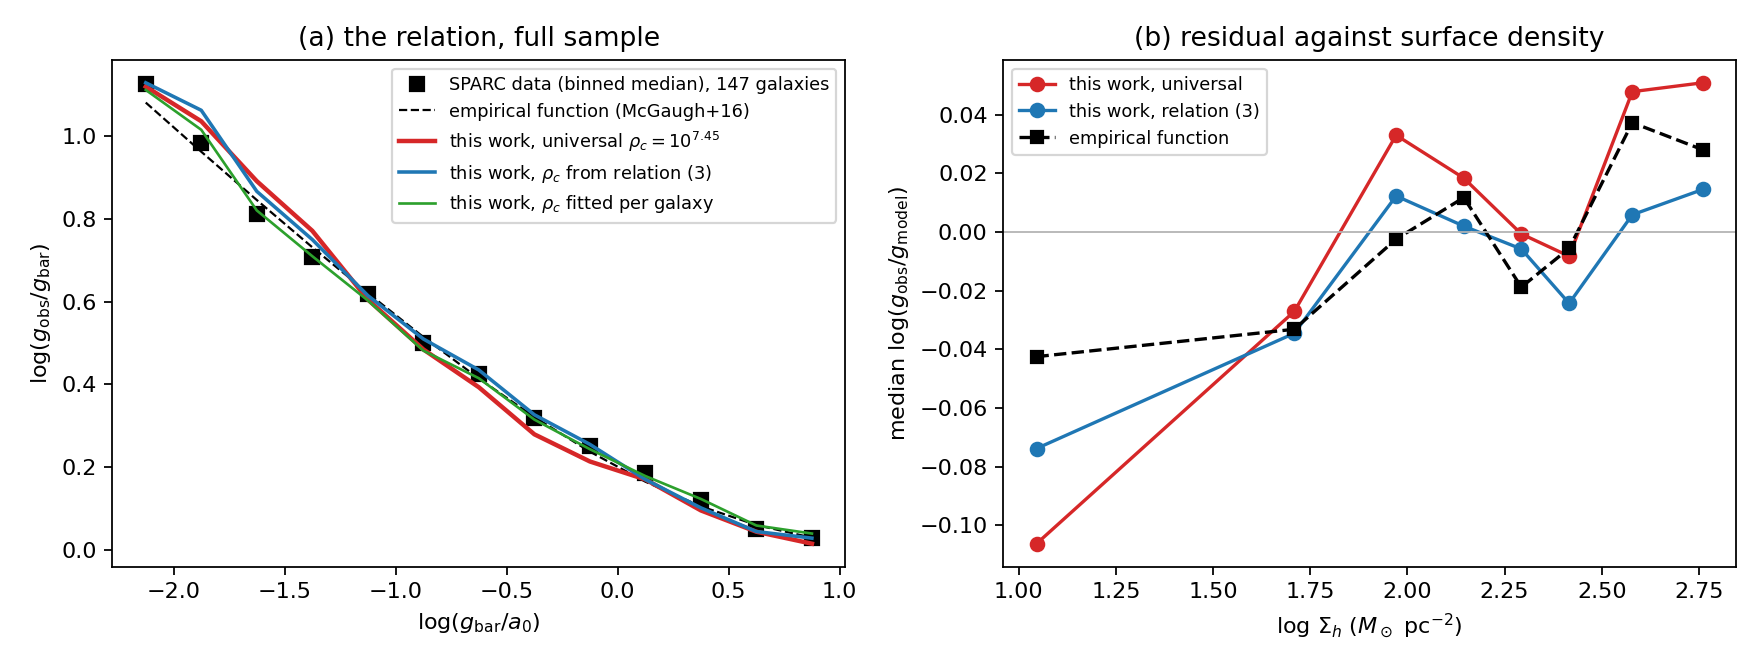
\includegraphics{figs_v2/fig1_emergent_nu.png}
\caption{(a) The radial acceleration relation on the full sample (147 galaxies, 2696 points; selection of McGaugh et al.~2016): binned data (squares), the empirical function (dashed), and eq.~(1) at the universal density $10^{7.45}$ (red), with $\rho_c$ from rule (3) (blue), and with $\rho_c$ fitted per galaxy (green). (b) The median residual $\log(g_{\rm obs}/g_{\rm model})$ in octiles of baryonic surface density $\Sigma_h$: eq.~(1) at universal density runs from $-0.10$ dex at the lowest surface densities to $+0.05$ at the highest, rule (3) halves that, and the empirical function itself is not flat ($-0.04$ to $+0.03$). Sensitivity to the saturation value is 0.07 dex per unit and to the form of $S$ up to 0.04 dex (Section 3).}
\end{figure}

Three honest limits of this result.
\begin{itemize}
\item[(i)] The normalisation is one global number taken from the data (the sample median); an independent choice, $\rho_c$ from the Donato et al.~core surface density, gives $10^{7.2}$ and lands within 0.1 dex of the data, uniformly low.
\item[(ii)] MOND predicts zero intrinsic scatter about the acceleration relation; eq.~(1) at universal $\rho_c$ predicts 0.07--0.11 dex at low accelerations, because galaxies with different baryon profiles reach different accelerations at the same $g_{\rm bar}$. The tightness of the acceleration relation is itself one of the regularities to be explained, so matching its mean is not enough. The intrinsic scatter has been measured: $0.034\pm0.001\,{\rm(stat)}\pm0.001\,{\rm(sys)}$ dex on SPARC, assuming the SPARC error model is reliable (Desmond 2023; Li et al.~2018 account for most of the observed 0.057 dex with errors); both this estimate and our error-injection test rest on that model, and uncertainties overstated in it would leave more room for intrinsic scatter. That estimate marginalises over mass-to-light ratio, distance and inclination, and our 0.07--0.11 dex is at fixed values, so the two are not directly comparable; but at the same baryon models the per-point rms of eq.~(1) exceeds the acceleration relation's by 0.08 dex in quadrature (0.155 against 0.133). A universal $\rho_c$ is therefore in tension with the data at fixed distances, inclinations and mass-to-light ratios. With those three free per galaxy within SPARC's quoted uncertainties (Gaussian priors as in Li et al.~2018), the tension is gone. Maximum-posterior fits give a per-point rms of 0.057 at the universal density, 0.057 with rule (3), 0.056 for the empirical function under the same treatment (Li et al.'s 0.057; Table 2's 0.067 for the same freedom is under the 10 per cent velocity weights of Section 3.2, not the quoted errors), and 0.045 with $\rho_c$ also free {[}RESULT\_MARG\_20261030{]}. Nested sampling over the same priors (147 galaxies; an intrinsic scatter of 0, 0.03 or 0.06 dex in $\log g$ as a further parameter) settles three questions a maximum-posterior fit cannot. First, the universal density and the empirical function prefer the same intrinsic scatter, 0.03 dex: the relation needs no more scatter than the empirical function does. Second, in Bayesian evidence the universal density is at least the equal of the empirical function: summed over galaxies, $\Delta\ln Z=+110\pm3$ in its favour at the preferred scatter, 0.7 per galaxy with a median of 0.2; at 0.06 dex the two are indistinguishable. Third, the distance shifts are comparable: 1.4 standard deviations rms for the universal density against 1.2 for the empirical function, 18 against 15 galaxies beyond 2 and 8 against 3 beyond 3. The maximum-posterior shifts of 2.0 rms, with IC 2574 moved by $-10$, were the mode, not the posterior; at the posterior median they are unremarkable. Freeing $\rho_c$ per galaxy is then strongly preferred: $\Delta\ln Z=+600$ over the universal density at the preferred intrinsic scatter, with the extra parameter's cost paid and distance, inclination and mass-to-light ratio marginalised (median $+0.13$ per galaxy; $+319$ from the galaxies with $|\Delta\ln Z|\le20$; $+1909$ at zero intrinsic scatter, which every model disfavours). The variation of $\rho_c$ is therefore information in the curves, not observational error absorbed by the fit, within SPARC's error model; errors understated by a factor of two would weaken that conclusion {[}RESULT\_NS\_20261030{]}. At low accelerations each galaxy's median offset from the data tracks how far its fitted $\rho_c$ lies from the one assumed (Spearman 0.85 at universal $\rho_c$ and 0.80 with rule (3) over the 113 galaxies with points below $a_0/10$; 0.91 and 0.89 over all points and all 147 galaxies). The central density relation of Lelli et al.~(2016c) says the same in observables (Appendix B.1). A density that varies with galaxy properties reduces the excess but does not remove it (rule (3): 0.140, 0.044 dex in quadrature, still above the measured 0.034); both quadrature figures subtract rms values of different models on the same points and are indicative only. Each galaxy is fit as well as by the empirical function with its mass-to-light ratio free (Table 2), and as well as by a feedback-cored $\Lambda$CDM halo with two parameters per galaxy (Section 3.2, Appendix B.3); what is not yet explained is why the central density varies with galaxy properties just enough to keep the relation tight. We state the two treatments of $\rho_c$ plainly: the universal value is the relation's reference, with no per-galaxy freedom, and it fails the central density relation (Appendix B.1); the per-galaxy value is a fit; the spread between them is the quantity the relation does not yet explain. The relation predicts neither the mean nor the width of that spread, which is what separates it from the concentration--mass relation of a $\Lambda$CDM halo, whose mean and 0.11 dex scatter are predicted independently of the curves.
\item[(iii)] At the single value eq.~(1) under-performs the empirical function in gas-dominated and slowly rising galaxies, where the fitted densities are lower (median $10^{7.19}$ for the galaxies without a flat part); that is where the low-acceleration offset comes from.
\end{itemize}


\subsection{3.2 Individual rotation curves, and the comparison with the acceleration relation}\label{individual-rotation-curves-and-the-comparison-with-the-acceleration-relation}

On the full sample the median per-galaxy $\chi^2$ is 25.5 at the universal density and 6.0 with $\rho_c$ free (Figure 2). The relation with its BTFR $\sigma$ does not describe individual curves to the data's precision; freeing $\sigma$ per galaxy roughly halves the median $\chi^2$ again (Appendix A.1).

\begin{figure}
\centering
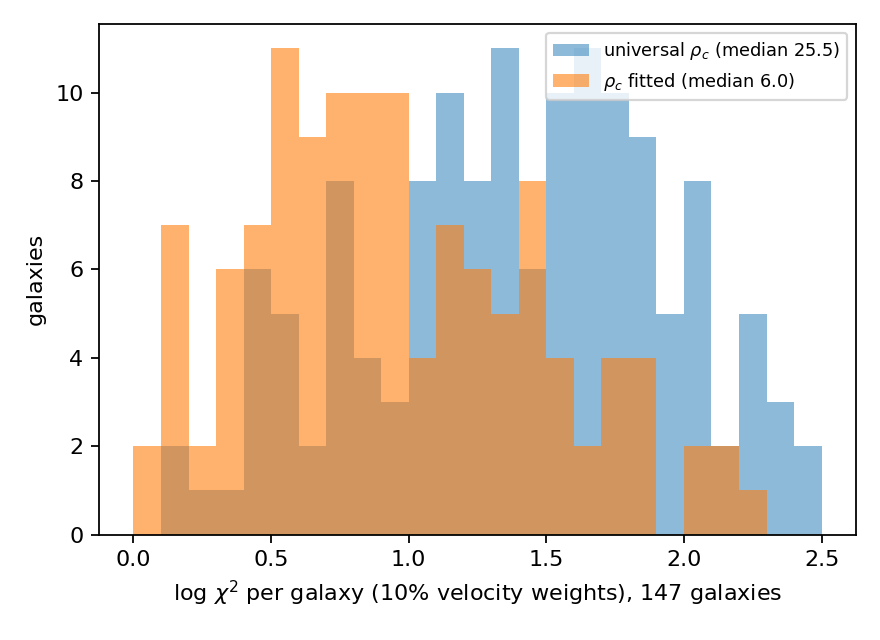
\includegraphics{figs_v2/fig2_chi.png}
\caption{Per-galaxy $\chi^2$ (10\% velocity weights) on the full sample at the universal density (median 25.5) and with $\rho_c$ fitted (median 6.0). The earlier three-way comparison (no saturation, saturated, $\sigma$ free) is given in Appendix A.1.}
\end{figure}

\begin{figure}
\centering
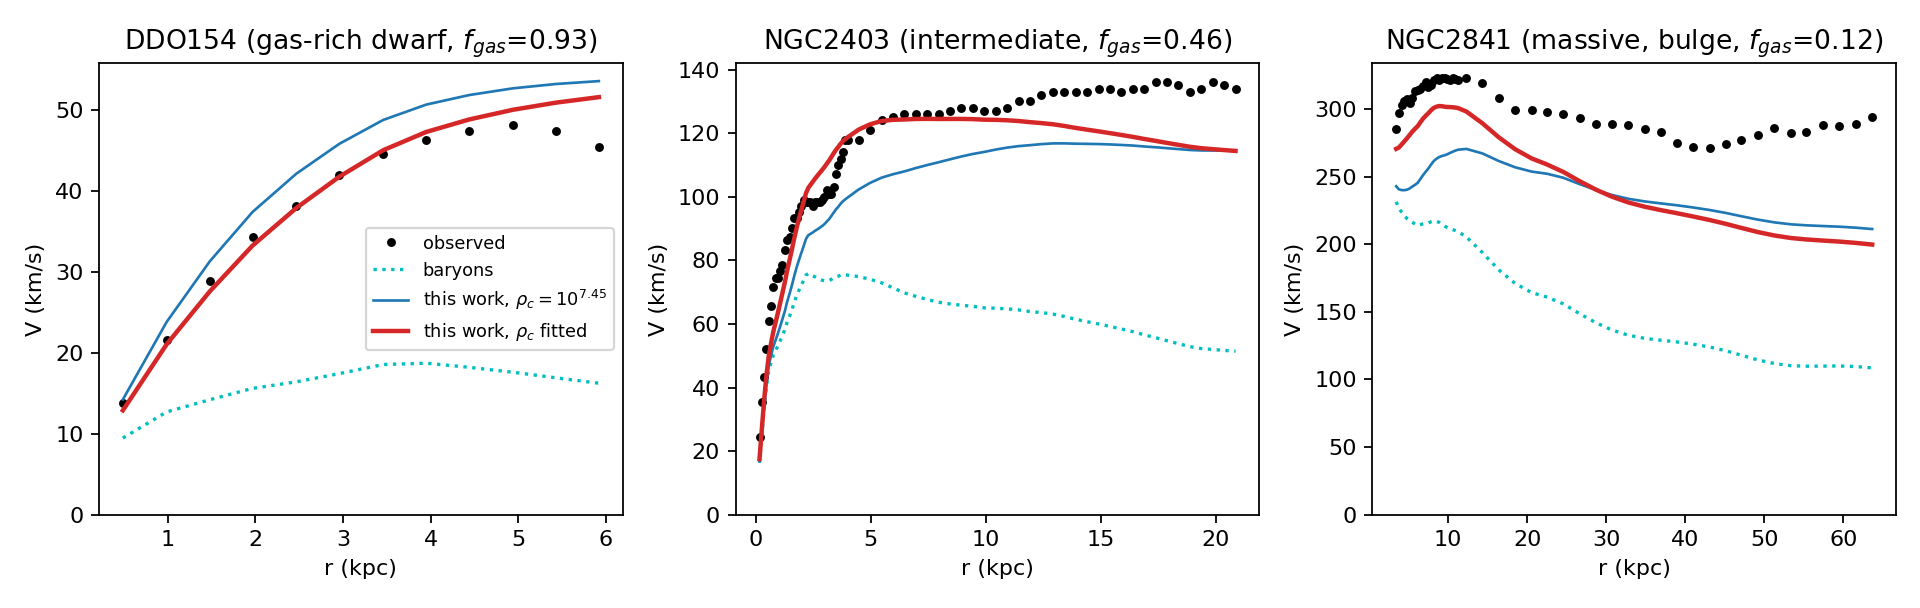
\includegraphics{figs_v2/fig3_curves.png}
\caption{Three rotation curves: observed (points), baryons (dotted), eq.~(1) at the single density $10^{7.45}$ (blue) and at the
fitted density (red). DDO 154 is gas-dominated; NGC 2403 intermediate;
NGC 2841 a massive bulge galaxy whose outer curve the relation under-predicts
by \textasciitilde{}25\% at either density -- the kind of residual that
the free-$\sigma$ fit of Appendix A.1 absorbs and the BTFR $\sigma$ does
not.}
\end{figure}

Table 2 places eq.~(1) and the empirical acceleration relation on the
same footing. On the full sample, per point, eq.~(1) at a single $\rho_c$ (0.155 dex) is worse than the empirical function at fixed M/L (0.133); with one free parameter each the two are equal within the noise (0.081 for eq.~(1) with $\rho_c$ free, 0.079 for the empirical function with the disc M/L free), and the empirical function with M/L, distance and inclination free under the SPARC priors reaches 0.067. The empirical function does slightly better in the galaxies without a flat part (0.072 vs 0.082). The fitted densities have median $10^{7.42}$ and spread 0.68 dex. (An earlier 120-galaxy comparison favoured eq.~(1), 0.108 vs 0.125; it does not survive the matched sample.) We draw no conclusion beyond ``comparable''. {[}pass2\_table2\_full\_20261022.py{]} For scale, self-interacting dark matter fits to SPARC carry two halo parameters per galaxy in addition to the mass-to-light ratio (Kaplinghat, Ren \& Yu 2020); this model carries one, with the mass-to-light ratio fixed. The comparison with $\Lambda$CDM halo models was then made under the nested-sampling machinery of Section 3.1, pre-registered, with distance, inclination and mass-to-light ratio marginalised identically for every model (Appendix B.3). Against an NFW halo with the cosmological concentration--mass prior (Dutton \& Macci\`o 2014; two parameters per galaxy) the relation with $\rho_c$ per galaxy is preferred by $\Delta\ln Z=+455$, and by $+338$ against NFW with the concentration free. Against the DC14 feedback-cored halo (Di Cintio et al.~2014) with the same prior, the fit is equal (summed maximum log-likelihoods differ by 5 over 147 galaxies) and the evidence favours the relation by $+65$, the Occam cost of a second halo parameter the curves constrain in one galaxy in ten (Appendix B.3); against a free Burkert halo the relation is preferred by $+146$ in evidence although the halo out-fits it by 97 in summed maximum log-likelihood: its two flat-prior core parameters cost more than they buy. The feedback core repairs NFW's failures in the low-surface-brightness galaxies (IC 2574, NGC 3109), as Li et al.~(2020) found, and keeps NFW's advantage in NGC 247, F571-8 and NGC 2403, where the relation loses 20--30 per galaxy. The halo reaches its fit with no galaxy's distance moved beyond two standard deviations; the relation with $\rho_c$ free moves twelve. At a single $\rho_c$ the relation loses to NFW by 146 and to DC14 by 536: with no per-galaxy freedom it is not competitive with a cosmologically primed halo on fit quality, and its claim there is economy and the predicted shape, not fit. We name the halo models rather than $\Lambda$CDM: the comparison is with one feedback prescription, and an abundance-matching prior on the halo mass, which a quarter of the DC14 posteriors would violate, was not imposed; it would lower the evidence for that quarter and could raise it elsewhere, so its net effect is not established {[}RESULT\_CDM\_20261031; RESULT\_CDM2\_20261031; RESULT\_CDM3\_20261031{]}. {[}RESULT\_N12 addenda
13:20-19:50{]}

Table 2. Per-point rms of $\log(g_{\rm obs}/g_{\rm model})$, 2696 points, 147 galaxies (selection of McGaugh et al.~2016).

\begin{longtable}[]{@{}lll@{}}
\toprule
model & free per galaxy & rms (dex)\tabularnewline
\midrule
\endhead
acceleration relation, M/L fixed & none & 0.133\tabularnewline
this model, $\rho_c=10^{7.45}$ & none & 0.155\tabularnewline
acceleration relation, M/L\_disc free & 1 & 0.079\tabularnewline
this model, $\rho_c$ free & 1 & 0.081\tabularnewline
acceleration relation, M/L, D, i free (SPARC priors) & 3 &
0.067\tabularnewline
(Li et al.~2018, MCMC, per-point errors) & 3 & 0.057 -- not
like-for-like\tabularnewline
\bottomrule
\end{longtable}

The Milky Way is a case the sample does not contain: a compact, massive disc whose Sun sits at about one MOND radius, and whose Gaia DR3 circular-velocity curve declines from 233 km/s at the Sun to \textasciitilde{}175 at 27 kpc (Ou et al.~2024). The relation is consistent with that decline, from their baryon model at the universal $\rho_c$ (rms 20 km/s over 8--27 kpc, slope $-1.9$ against the observed $-2.5$ km/s/kpc), within 3 km/s of MOND on the same baryons at every radius; with $\rho_c$ fitted ($10^{7.88}$, inside the sample spread) the rms is 9 km/s (slope $-3.0$ against the observed $-2.5$). The decline is the transition toward the BTFR speed of 177 km/s, not a Keplerian fall: at the Sun the baryons alone give 173 km/s and the nb mass the rest. Appendix A gives the numbers and the outer prediction. {[}RESULT\_MW\_DECLINE\_20261021{]}

\subsection{3.3 The core surface density}\label{the-core-surface-density}

MOND obtains the halo core surface density from $a_0$ (Milgrom 2009). In galaxies whose mean acceleration is at or above $a_0$ it is $\gamma\Sigma_M$, with $\Sigma_M=a_0/2\pi G\approx138\,M_\odot\,{\rm pc}^{-2}$ and $\gamma$ of order unity, fixed by the interpolating function. At low surface density it falls as $\sqrt{\Sigma_b}$. Donato et al.~(2009) measure log $\mu_0$ = 2.15 $\pm$ 0.2. The fitted $\rho_c$ of this relation implies a median log $\mu_0$ = 2.24 $\pm$ 0.39, with $\mu_0=\rho_c r_c$: reproduced on average, not predicted. $\mu_0$ is not a parameter of eq.~(1): with $r_c=3\sigma/\sqrt{4\pi G\rho_c}$ it is $3\sigma\sqrt{\rho_c/4\pi G}$, so at a universal $\rho_c$ it rises as $M_b^{1/4}$, and the fitted $\rho_c$ remove most of that rise. Figure 4 compares the two galaxy by galaxy. MOND's value is Milgrom's estimate (his eq. 11), which he calls rough. We evaluate it with the interpolating function of the acceleration relation, which gives $\gamma=2.09$, and with $\Sigma_b$ the mean baryonic density inside the half-mass radius times that radius ($\Sigma_b=0.75\,\Sigma_h$). Against baryonic mass the SPARC Burkert fits of Li et al.~(2020) rise with slope +0.21. This relation's values rise with +0.24. MOND's rise with +0.15 (+0.13 to +0.16 with $\Sigma_b$ halved or doubled). Fitted on mass and surface density together, the Burkert values go as $M_b^{0.14\pm0.04}\Sigma_h^{0.20\pm0.07}$ and this relation's as $M_b^{0.16\pm0.05}\Sigma_h^{0.22\pm0.07}$. MOND's depend on $\Sigma_b$ alone, as $\Sigma_h^{0.40}$, with no mass term.

Galaxy by galaxy the rms offset from the Burkert values is 0.26 dex for this relation and 0.30 for MOND (109 galaxies in both). Two cautions keep this from being a discriminator. First, this relation's values come from one density fitted per galaxy to the same rotation curves the Burkert fits use, so the agreement is partly shared input; MOND's values carry no per-galaxy freedom. Second, the mass trend depends on the mass-to-light ratio. At a disc M/L of 0.7, or a mass-dependent one, $\rho_c$ falls with mass (slope $-0.26$ to $-0.30$) and the implied $\mu_0$ slope drops to \textasciitilde{}0.12 {[}RESULT\_TEST1 addendum 17:25{]}; MOND's slope at that M/L was not recomputed. We read the comparison as Table 2 reads the rotation curves: a comparable description with a different parameter count. What the relation lacks is in the amplitude of the tail, which it sets by $M_b$ alone (Section 4.1). {[}fig4\_mu0\_mond\_20261027.py; RESULT\_FIG4\_MU0\_MOND\_20261027{]}

\begin{figure}
\centering
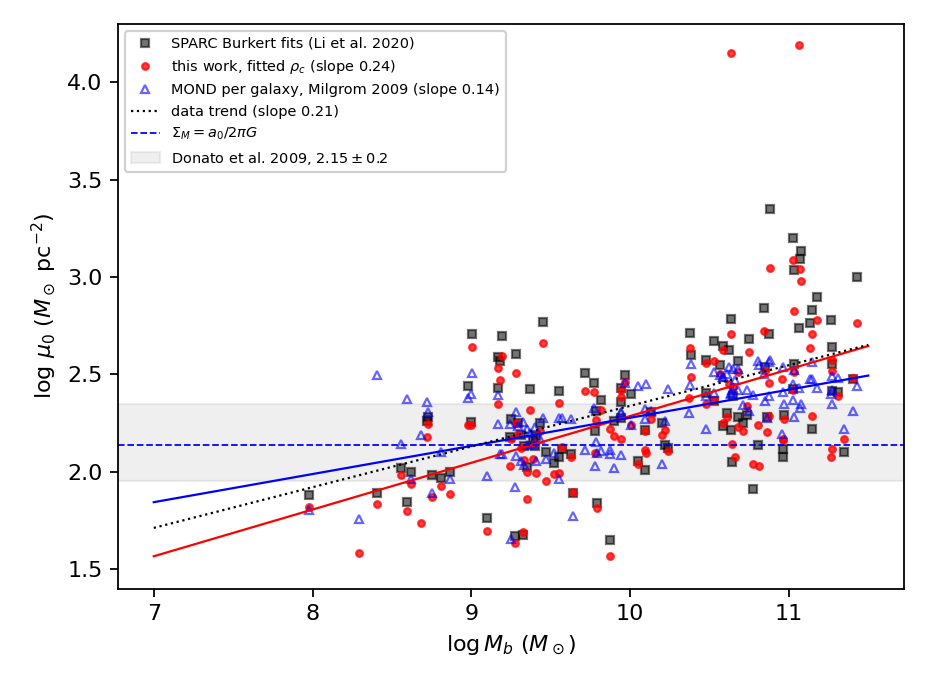
\includegraphics{figs_v2/fig4_mu0.png}
\caption{Halo core surface density $\mu_0$ against baryonic mass, 120 SPARC galaxies at the SPARC mass-to-light ratio. Squares: Burkert fits to the data (Li et al.~2020); dotted line, their trend. Red points: this work, $\mu_0=\rho_c r_c$ with $\rho_c$ fitted per galaxy and the King radius $r_c=3\sigma/\sqrt{4\pi G\rho_c}$; this is a King core, not a Burkert refit, so the comparison with Burkert $\rho_0 r_0$ is approximate. Open triangles: MOND's value for each galaxy from its baryons (Milgrom 2009, eq. 11), with the interpolating function of the acceleration relation ($\gamma=2.09$) and $\Sigma_b=0.75\,\Sigma_h$. Solid lines: least-squares trends. Dashed: $\Sigma_M=a_0/2\pi G$. Band: Donato et al.~(2009), $2.15\pm0.2$. The red points use one fitted density per galaxy; the triangles use none (Section 3.3). {[}fig4\_mu0\_mond\_20261027.py{]}}
\end{figure}

\section{4. Where the model is incomplete}\label{where-the-model-is-incomplete}

\subsection{4.1 Surface-density dependence at fixed mass}\label{surface-density-dependence-at-fixed-mass}

The dependence on surface density at fixed baryonic mass, which MOND predicts, is present in the data. In the relation it is missing from the tail, whose amplitude $\sigma$ is set by $M_b$ alone. (The fitted $\rho_c$ does depend on surface density -- Section 3.3 and rule (3) -- but $\rho_c$ sets the core, not the tail.) It shows directly in the outer curves: at the single density the ratio of model to observed speed at the last measured point has median 1.02 over 147 galaxies, with no trend in baryonic mass but a clear one in surface density (Spearman $-0.30$, $p=2\times10^{-4}$), from 1.085 in the lowest-surface-density quartile to 0.98 in the highest. The excess does not correlate with inclination, inclination error or distance error, but it does shrink with data quality: in the 69 galaxies with quality flag 1, inclination $\ge45^\circ$ and inclination error $\le5^\circ$ the trend is not significant (Spearman $-0.15$, $p=0.22$) and the lowest-quartile excess is 4\%, against $-3$\% in the highest.

Correcting the outer speeds for pressure support in the gas (asymmetric drift; gas dispersion 6--12 km/s, as measured in dwarfs and outer discs by Ianjamasimanana et al.~2015 and Iorio et al.~2017; exponential outer gas disk) removes about a third of the lowest-quartile excess at the universal density (8.5\% to 5.5\% at 8 km/s) and little of it under rule (3); with the drift term and $V_{\max}$ controlled, the surface-density term survives at 2.4$\sigma$. {[}pass4\_oman\_drift\_20261022.py; RESULT\_PASS4\_OMAN\_DRIFT\_20261022; VERIFY whether some SPARC dwarf curves are already drift-corrected{]} We read it as a residual of 3--8\% with MOND's sign, partly data quality and partly pressure support; it tracks gas fraction, and it is not removed by any choice of $\rho_c$ (Section 3.1), so it sits in the amplitude of the tail, which the relation fixes by $M_b$ alone.

The stellar mass-to-light ratio does not absorb it: at a disc M/L of 0.4, 0.5 and 0.7 the lowest-quartile excess is 5, 8 and 13\% and the highest-quartile ratio 0.94, 0.98 and 1.09, so a higher M/L narrows the differential only by over-predicting every galaxy, and the low-acceleration offsets grow with M/L; 0.5, the population-synthesis value (Schombert, McGaugh \& Lelli 2019), gives the best rms of the three {[}pass3\_ml\_sensitivity\_20261022{]}. Freeing the velocity parameter per galaxy shows where the residual lives: the BTFR value is right on average (median offset $-0.006$ dex in $\sigma^2$), and the fitted offset tracks gas fraction ($-0.49\pm0.15$ per unit $f_{\rm gas}$), not surface density, once both are included. Setting $\sigma$ by the baryonic mass enclosed within the last measured point, instead of the total, removes the gas-fraction trend and most of the low-surface-density excess, but a velocity parameter that depends on radius is a different relation (Section 7) and is not attempted here. The isothermal form also overshoots its asymptote near three core radii, and the residuals at the last point show that hump (peak at $R\approx2.8\,r_0$, $3\sigma$), independent of the surface-density trend. {[}RESULT\_PASS5\_SIGMA\_FREE\_OVERSHOOT\_20261022; RESULT\_PASS6\_LOCAL\_SIGMA\_20261022{]} Over the galaxies with a flat part the relation reaches $V_f$ as the data do (median model 1.002, observed 1.006 of $V_f$ at the last point), so the shortfall seen in individual massive discs (Figure 3) is not a sample property. {[}RESULT\_PASS2\_SPARC\_FULL\_20261022{]} {[}TEST1b; test1e{]}


\subsection{4.2 Crater II}

McGaugh (2016) predicted $\sigma$ = 2.1 (+0.9/-0.6) km/s from the external-field effect before Caldwell et al.~(2017) measured 2.7 $\pm$ 0.3. At $\rho_c=10^{7.45}$ the relation gives 5.2 km/s; it reaches 2.7 only with $\rho_c\sim 10^{6.1}$, 1.3 dex below the median {[}RESULT\_RHOC\_SIGMA\_B\_OOS{]}. The surface-density trend alone ($\rho_c$ against $M_b$ and $\Sigma_h$) supplies a third of that, predicting $10^{7.0}$; the full rule (3), in which the gas-fraction term raises $\rho_c$ for a gas-free object, predicts $10^{8.7}$, i.e.\textasciitilde{}it moves the wrong way; the dispersion there is 5.1-5.4 km/s because above $\sim 10^{7.5}$ the projected dispersion saturates near the relation's velocity parameter (5.7 km/s for Crater II) {[}RESULT\_DWARF\_PREREG; RESULT\_RHOC scan{]}. Crater II's tidal disruption has been reported (Vivas et al.~2026). Quantified under the relation, with its own Milky Way curve and the pericentre of Ji et al.~(2021), 21.7 kpc, truncation at the pericentric Jacobi radius brings the universal-$\rho_c$ value to 3.1--2.8 km/s, within the bar of Caldwell et al.\ and, in the stronger case, of Ji et al.'s 2.34 km/s; Antlia II, observed to be disrupting, passes in the same cases (Appendix B). Because that radius (0.7 kpc) lies inside today's half-light radius, these are bounds, not a model; a stripping calculation is owed. The mechanism is the tidal one CDM uses (Sanders, Evans \& Dehnen 2018; Borukhovetskaya et al.~2022). Status: conceded at equilibrium; the tidal reading is listed as open until a stripping calculation exists (Section 7). {[}RESULT\_CRATER2\_TIDES\_20261021{]}

\subsection{4.3 NGC 1052-DF2 and DF4}

Both have stellar dispersions consistent with
their stars alone: 8.4 $\pm$ 2.1 km/s (Danieli et al.~2019) and 8.0
(+2.3/-1.9) (Shen et al. 2023), at 20-22 Mpc (Shen et al.~2021), with
$M_*\sim 2\times10^8$ (van Dokkum et al.~2018) and
$\sim1.5\times10^8\,M_\odot$ (Shen et al.~2023 adopt $M_*=7.5\pm2\times10^7$ inside the 3-D half-light radius at M/L = 2, from van Dokkum et
al.~2019; their dynamical mass there is $8\,(+6/-4)\times10^7$ against a
stars-only expectation of 7 $\pm$ 1 km/s) {[}BALLOT VERIFY LEDGER
2026-10-20 20:05{]}. The relation at the sample density gives 17-22 km/s; it
needs $\rho_c$ about 1.5 and 1 dex below the SPARC galaxies of the same
mass and surface density, which is not an extrapolation of rule (3)
but an outlier to it. The relation has no lever here. They are anomalous for
isolated MOND as well (\textasciitilde{}20 km/s); MOND recovers 13.4
(+4.8/-3.7) through the external field of NGC 1052 at a separation not
known in three dimensions (Famaey, McGaugh \& Milgrom 2018; Haghi et
al.~2019). We list them as unexplained because the relation has no comparable
lever, not because MOND predicts them.

\subsection{4.4 Environment}

The relation predicts that the shape of a rotation curve
does not depend on the external field of neighbouring galaxies: the ambient density at a field galaxy is \textless{}\textasciitilde{} 630 $M_\odot$ kpc\^{}-3 (Appendix C {[}RESULT\_N10{]}) against a core density
$\sim 10^{7.5}$, and the nesting boost is \textasciitilde{}1
{[}NEST-1{]}. On SPARC the low-acceleration residual from the
acceleration relation varies with the environmental field of Chae et
al.~(2021) as -0.12 $\pm$ 0.16 dex per dex at fixed mass and surface
density; the external-field effect predicts -0.08 for this sample, the
relation 0; the sample does not separate them. Applying their own statistic
(a fitted external-field parameter per galaxy) to the relation's curves
returns a positive median too, so their median detection does not
discriminate the relation; the dependence of that parameter on the field is
weak and not of the external-field sign on the galaxies with field
values; their cosmic-web regional contrast is untested here. Appendix D.
This is the note's open weak point.

Three of these (4.2-4.4) are one problem stated three times: the relation's
environmental effect is enhancing and small, so wherever MOND explains a
low dispersion by suppression from an external field, this relation must
explain it with a low $\rho_c$ or need no suppression at all -- And XIX needs none (the universal value gives 8.3 km/s against 7.8 observed, Appendix A), but the relation does not supply a low enough $\rho_c$ for
Crater II (the surface-density trend alone goes a third of the way; the full relation does not; a tidal reading is open, Section 7), and not for DF2 and DF4.

\section{5. What real mass buys}\label{what-real-mass-buys}

The three purchases of the introduction, with their evidence in Appendix
C: lensing and dynamics from the same mass (it lenses as ordinary mass),
compatible with the flat isolated-galaxy profiles of Mistele et al.~(2024b) to 1 Mpc, with a truncation predicted at 0.8--3.4 Mpc for an isolated $L^*$ galaxy, and a Mpc-scale budget that is open, with a mean-field indication that it can close (Appendix C);
no suppressing external-field effect (the environmental coupling is
small and enhancing); and a present-tense relation, so that identical baryons
today give identical nb mass whatever came before.

The ambient term does four things at once:
\begin{itemize}
\item it truncates each halo where the tail meets the local nb density, so the cut tracks environment through density rather than through an external field;
\item it keeps the downturn in voids, at larger radii;
\item it carries no external-field suppression of internal dynamics;
\item and it makes the force between bodies farther apart than their truncation radii inverse-square, as the pairwise kinetic Sunyaev-Zel'dovich measurement finds (Gallardo et al.~2026; Appendix E).
\end{itemize}
These, not the galaxy-scale fits, are where the
relation and MOND part.

Positivity. In MOND's field formulations the phantom density turns
negative in a region around the point where an embedded system's internal
field cancels the external one (Milgrom 1986). For MOND this is harmless,
since the phantom density is not mass. For a theory in which the missing
mass is real it is a constraint: real mass cannot be negative, so such a
theory cannot follow MOND there. This relation has no phantom density: the extra mass is real nb mass, positive everywhere, and the departure is a prediction: Newtonian dynamics for wide
binaries in the Galactic field, provided their own central density stays
low (Section 6.1). The argument does not show that
MOND fails; it shows where a real-mass account must differ from it.

\section{6. Predictions and falsifiers}\label{predictions-and-falsifiers}

\subsection{6.1 Wide binaries}

Status: live; the Newtonian value is shared with Newton and $\Lambda$CDM, so this test discriminates against MOND only. Let $\gamma$ be the ratio of the observed to the Newtonian relative acceleration of a wide pair at given separation. A wide binary is a body like any other (Section 2.3); it is Newtonian not because it lacks nb mass but because the nb density is bounded, so the mass inside its orbit is negligible. Because the response density is bounded above by $e^2\rho_c$ -- below a few solar masses per cubic parsec for any fitted $\rho_c$ -- a wide binary encloses a negligible nb mass: for a 2 $M_\odot$ pair at 7--28 kAU, $\gamma-1=2\times10^{-5}$ to $2\times10^{-3}$, under either choice of velocity parameter and in the halo as in the disc. To reach $\gamma$ = 1.1 at 28 kAU would require 19 $M_\odot\,{\rm pc}^{-3}$ inside the orbit, two decades above any density on file.

The relation predicts $\gamma$ = 1.000 (+\textless{} 0.003) provided the binary's own central density is below $\sim10^{10}\,M_\odot\,{\rm kpc}^{-3}$ ($\gamma-1<0.1$ at 28 kAU); the globular-cluster bound ($\lesssim10^{7.2}$, Appendix A) clears this by three decades, and rule (3), calibrated on discs, does not extend to stellar systems. Conversely, Newtonian data at 1\% precision would bound it below $10^{9.2}$. {[}pass9\_wb\_rhoc\_sweep\_20261025.py; RESULT\_SIMROUND\_C1-C4 C3{]} We state in advance what is being tested: eq. (1) with the central density of stellar systems bounded by the globular-cluster value. A confirmed $\gamma\ge1.1$ falsifies that model; raising the binary's density afterwards to $\sim10^{10}$ would be a new hypothesis, not a rescue of this one. A variant in which the host's nb mass is depleted around the pair, keeping the total non-negative, gave $\gamma\approx1.1$--1.25 (Appendix F); it is a different relation from eq. (1), and DR4 separates 1.00, $\sim$1.2 and 1.3. MOND with the Galactic external field predicts $\gamma$ = 1.28-1.36 at separations of 1-4 MOND radii, i.e.\textasciitilde{}7-28 kAU for a 1 $M_\odot$ system and 10-40 kAU for 2 $M_\odot$ {[}RESULT\_WB\_R1PC{]} (two-body QUMOND formalism: Pflamm-Altenburg 2025); the relation's $\gamma$ - 1 \textless{} 0.003 holds across that range.

The present data are disputed. Cookson et al. (2026), Banik et al.~(2024) and Pittordis et al.~(2025) find Newtonian behaviour at all separations (Newton up to 1500x more likely than MOND in the cleanest sample of Cookson et al.). Chae (2023, 2024a,b, 2025) reports a boost at $g_N\lesssim10^{-9}\,{\rm m\,s^{-2}}$ ($\gamma_g\approx1.3$--1.5), with Newton rejected at 5--10$\sigma$ in his samples, and Chae et al.~(2026) find $\gamma=1.60^{+0.24}_{-0.14}$ in 36 systems with accurate 3-D velocities; Hernandez et al.~(2024) also report a boost; and Chae \& Yoon (2026) argue that the data-quality cuts used by Banik et al.~and Cookson et al.~bias the result toward Newton.

The relation's $\gamma$ = 1.000 is therefore already disfavoured by one side's analyses and consistent with the other's. The falsifier we commit to is a confirmed $\gamma$ $\ge$ 1.1 from Gaia DR4 under a selection both sides accept: an error cut on the projected velocity in ${\rm m\,s^{-1}}$ rather than on the scaled velocity, a multiplicity fraction calibrated in the Newtonian regime of the same sample, hundreds of pairs beyond one MOND radius, and a stated $\gamma$ convention. The MOND reference values above are a two-body QUMOND calculation at fixed separation, benchmarked against the independent two-body solutions of Pflamm-Altenburg (2025) to within 0.03 at 7-28 kAU; his finding that the one-body (test-particle) approximation overstates the boost (up to 1.44 against 1.2-1.3) applies to analyses that use it, not to these values. {[}RESULT\_FRM3\_WB\_FROZEN\_LAW{]}

\begin{figure}
\centering
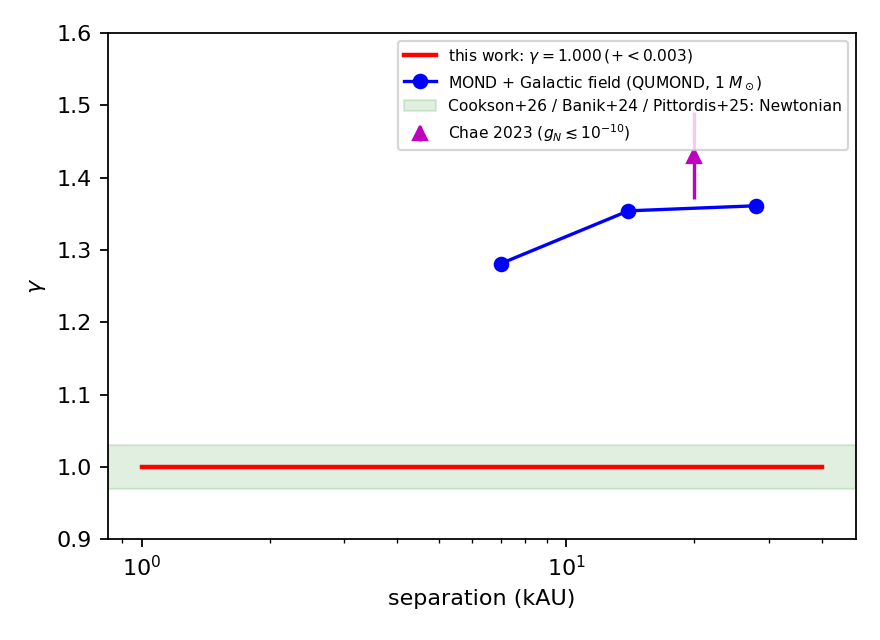
\includegraphics{figs_v2/fig5_wb.png}
\caption{Wide binaries: the relation predicts $\gamma$ = 1.000
(+\textless{} 0.003) at all separations for binary central densities below $\sim10^{10}\,M_\odot\,{\rm kpc}^{-3}$ (red); MOND with the Galactic
external field, two-body QUMOND for a 1 $M_\odot$ system, gives 1.28-1.36
(blue; separations scale with ${\rm mass}^{1/2}$). The green band marks the
Newtonian results of Cookson et al.~(2026), Banik et al.~(2024) and
Pittordis et al.~(2025); the magenta point is Chae (2023). The status of
these data is disputed (Section 6.1).}
\end{figure}



\subsection{6.2 Environment}

Status: live; paired with 6.1, opposite MOND expectations.
Observable: the mean residual $\log(g_{\rm obs}/g_{\rm RAR})$ over points with $g_{\rm bar}$
\textless{} $a_0$/3, per galaxy, against the maximum-clustering
environmental field log $e_N$ of Chae et al.~(2021), at fixed log $M_b$
and log $\Sigma_h$. The relation predicts slope 0; the external-field effect
predicts -0.08 dex per dex for the SPARC sample. A slope of -0.08 $\pm$
0.03 or tighter on a larger sample falsifies the relation's environmental
prediction and, with it, the source rule of Section 2.3. {[}RESULT\_N8B
addendum{]}

\subsection{6.3 The ambient truncation}

Status: live (Appendix C, Figure 7). The stacked lensing circular velocity of isolated galaxies turns down at $r_t=\sigma/\sqrt{2\pi G\rho_{\rm amb}}\propto M_b^{1/4}\rho_{\rm amb}^{-1/2}$, with, for isolated galaxies, one $\rho_{\rm amb}$ for every mass bin, the most massive bin last, and $v_c\propto r^{-1/2}$ beyond. The mass ordering is not by itself a discriminator: an external-field decline in MOND sets in where the internal field falls to the external one, at a radius $\propto M_b^{1/2}$ at fixed field, more steeply mass-ordered than $M_b^{1/4}$; massive galaxies also sit in denser surroundings, so $\rho_{\rm amb}$ correlates with $M_b$; and the two-halo term is mass-ordered too.

What distinguishes the two is the shape (a cut at an ambient density against a roll-over set by the external field) and the dependence on environment at fixed mass; the separation must be shown with mock stacks and an orientation-averaged external-field profile, neither of which is done here. The value of $\rho_{\rm amb}$ is the one free parameter of the forecast. The data within 1 Mpc bound it from above only ($<630$--$710\,M_\odot\,{\rm kpc}^{-3}$ at 95\%, depending on the radial range fitted, and 160--355 with the amplitude fixed by the relation; Appendix C); the points beyond 1 Mpc mildly prefer a truncation, but the ambient density they would imply ($\sim$350, nine times the cosmic mean around galaxies selected as isolated) would itself lens and is not credible, so we do not quote it as a fit. The closure identity $a_0^2/Gc^2=35.5$ ($r_t\approx3.4$ Mpc for $L^*$) is the one physically motivated value, and the forecast below is stated for it and for the bound.

A forecast with $V_f$ free, the covariance of the deprojected points, the extrapolation systematics and a two-halo nuisance term is owed and not attempted here; qualitatively, a truncation at the bound (0.8 Mpc for $L^*$) is already within reach of present data if the two-halo term can be controlled, and the closure value (3.4 Mpc) is beyond isolated-lens selection; the closure value needs 5 Mpc, beyond where isolated-lens selection holds against the two-halo term. Outcomes: a decline with the predicted shape and a common $\rho_{\rm amb}$ across mass bins detects the ambient term and measures it; flatness to 2 Mpc at better precision pushes $\rho_{\rm amb}$ below $\sim$60 and leaves the closure value untested; a decline that follows environment at fixed mass rather than a common ambient density favours the external-field reading. Lensing flatness alone is therefore not a falsifier of the relation; flatness to 5 Mpc at the forecast precision falsifies the closure value of the ambient density for isolated galaxies (Section 6.5), not eq. (1). {[}euclid\_forecast\_20261021.py; RESULT\_LENSING\_FIT\_SATELLITES{]}

\subsection{6.4 Further predictions}

One test has already been made against a quantity not derived from rotation curves. The DiskMass Survey measures the stellar vertical velocity dispersions of 30 face-on spirals and from them the baryonic fraction of the rotation at $2.2h_R$, $\mathcal{F}_b=V_b/V_c=0.57$ (median), independently of the rotation curve (Bershady et al.~2010; Martinsson et al.~2013a,b). Solving eq.~(1) at the universal $\rho_c$ for each galaxy's baryonic mass and scale length predicts $\mathcal{F}_b=0.66$ (median), 0.09 above the measurement with 0.13 rms and nothing fitted; MOND, with no halo, predicts 1 (Angus et al.~2015). The offset has the sign expected if these spirals carry $\rho_c$ above the universal value, as their SPARC analogues do; the DiskMass inclinations are Tully--Fisher based, and the dispersions have been argued to be biased low by young stars (Aniyan et al.~2016), which would raise the measured value {[}RESULT\_DMS\_20261105{]}.

Three predictions are detailed in Appendix E:
\begin{itemize}
\item the starless cloud Cloud-9 is bound only if its own nb mass is large enough ($\log\rho_c\gtrsim6$, giving $1$--$7\times10^7\,M_\odot$ inside 1.4 kpc, of the order its line width implies);
\item early- and late-type lensing relations identical at fixed baryonic mass under the dynamical assumption of Section 2.2, whereas a conserved completion predicts an early-type excess growing with merger history (about 0.04--0.075 dex in $g_{\rm obs}$ per merger); the data show a $\ge6\sigma$ difference in Brouwer et al.~(2021) and none significant after the stellar-mass, hot-gas and isolation corrections of Mistele et al.~(2024a,b), who recover Brouwer's difference with Brouwer's choices;
\item the pairwise force law at 30-230 Mpc.
\end{itemize}
No dynamical friction from the nb mass, under the dynamical assumption of Section 2.2 (not a consequence of the relation): its response is fast compared with the bar's rotation, so a bar rotating through it leaves no lagging wake and loses no angular momentum to it. Fast bars ($\mathcal{R}=R_{\rm CR}/R_{\rm bar}\approx1$) are then expected, as in MOND; in $\Lambda$CDM simulations halo friction slows bars (Debattista \& Sellwood 2000), a tension reported at $>9\sigma$ for EAGLE and IllustrisTNG by Roshan et al.~(2021) and reduced in the more baryon-dominated Auriga discs by Fragkoudi et al.~(2021). Shared with MOND; a discriminator against massive dynamical haloes only.

\subsection{6.5 Tests in reach}

The predictions above can be tested with data that exist or are scheduled; we state each with its main systematic so that each is decidable.
\begin{itemize}
\item[(i)] Lensing beyond 1 Mpc. Stacked galaxy-galaxy lensing to $\sim$5 Mpc, binned by baryonic mass and by local density measured from spectroscopic redshifts (DESI overlapping KiDS or HSC now; Euclid later). The relation predicts a downturn whose radius scales as $M_b^{1/4}\rho_{\rm amb}^{-1/2}$: about 3--6 Mpc across the four mass bins of Mistele et al.~(2024b) at the closure density (Appendix C), with the excess surface density at 5 Mpc falling to 0.49--0.91 of the untruncated profile (for baryonic masses 0.1 dex above nominal, as the lensing amplitude prefers); at an ambient density of 160 the downturn moves to 1.4--2.7 Mpc. The radius ratio between the heaviest and lightest bins is about 1.8 (3.2 to 5.9 Mpc), against about 3.4 for a decline set by MOND's external field at fixed field strength (radius $\propto M_b^{1/2}$), and the relation's radius follows the ambient density rather than the field. Because the ambient density is set by a smooth background field rather than by the surrounding galaxies, the downturn persists in voids, at larger radii where the background lies below its global mean, while MOND's external-field decline recedes. Main systematic: the two-halo term, which must be forward-modelled on mocks with the same selection. Falsified by: flatness to 5 Mpc at the closure precision (which falsifies the closure value for isolated galaxies, not eq. (1)), or a radius ratio near 3.9. {[}pass11\_lensing\_forecast\_20261025.py{]}
\item[(ii)] Wide binaries (Gaia DR4). $\gamma=1.00$, provided the binary's own central density is below $\sim10^{10}\,M_\odot\,{\rm kpc}^{-3}$ (Section 6.1). Main systematic: quality cuts and hidden companions. Falsified by: a confirmed $\gamma\ge1.1$ (of eq. (1) with the globular-cluster density bound, declared in Section 6.1).
\item[(iii)] Dwarfs, predictions first. For dwarfs without measured dispersions, the relation's and MOND's (with the external field) predictions are to be published before the data, under the protocol of Appendix B (its first pass is reported there). The relation predicts embedded and isolated dwarfs alike; MOND predicts the embedded ones lower. Main systematic: tides and non-equilibrium. Falsified by: embedded dwarfs below isolated ones by more than 0.15 dex on average.
\item[(iv)] Bars. With no friction from the nb mass under the dynamical assumption (Section 2.2), bars stay fast (Section 6.4). Main systematic: pattern-speed measurement (Tremaine-Weinberg). Falsified by slow bars as the norm -- which would falsify the dynamical assumption, not the relation.
\end{itemize}
Beyond these, planned SKA-Mid HI surveys would raise rotation-curve samples from a few hundred galaxies to tens of thousands, across environments and to $z\sim1$ (Lelli et al.~2026). They would test the environment prediction of Section 6.2 on rotation curves directly, and the BTFR normalisation of the tail (eq.~2) at low mass, where few present curves reach their flat part.



\section{7. Open list}\label{open-list}
\begin{itemize}
\item $\rho_c$: what sets it (solution selection). This is the first open item. Five rules tried (rule (3), the central density relation imposed, the background normalisation, MOND's central-surface-density bound, a universal value) hold the population slope at best and none holds the per-galaxy values; the fitted values track no baryon property and trade against the mass-to-light ratio and distance (Appendix B.1). The conclusion that $\rho_c$ is information rather than absorbed error rests on SPARC's quoted distance and inclination errors (Section 3.1). Until a rule exists, the relation's advantage over a two-parameter halo is a parameter count, not a prediction.
\item The halo comparison (Appendix B.3) owes a DC14 arm with an abundance-matching prior on the halo mass, and a cored-halo arm in the dwarf protocol.
\item Structure formation before recombination: out of scope and acknowledged (Section 1). Two routes may be named, neither calculated: the background field of Section 2.1 carrying linear perturbations of its own, in which case the early universe is $\Lambda$CDM's and the relation describes the non-linear, galaxy-scale regime; or the relation's own linear response amplifying baryon growth after recombination.
\item The extended-gas source: how much nb mass a cloud carries is set by its $\rho_c$ (Section 2.3), which is not understood; tested by Abell 520 (a gas-centred lensing core, if confirmed on undisputed data, contradicts it) and Cloud-9.
\item The nesting rule: the LMC carries a 1.67x excess of Milky Way nb mass at its centre ($1.2\times10^9\,M_\odot$ within 30 kpc). The body decomposition is stated, not derived (Section 2.3): a body's components enter only through its $\varphi_b$, a self-bound satellite is a body with its own $\sigma$; a truncation of satellite haloes where the host's field dominates was tested and rejected -- it reproduces MOND's external-field pattern on the diffuse satellites (Crater II recovered, And XIX lost) and cuts the LMC further.
\item Galaxy clusters: counting the hot gas as part of the cluster body (Section 2.3), the relation reaches MOND parity inside 2 Mpc for a Coma-like cluster ($7\times10^{14}\,M_\odot$ of nb against $\sim8.5\times10^{14}$ needed) and keeps MOND's inner-Mpc deficit; the nb released by member galaxies is about three-quarters of the cluster's own halo out to its truncation radius, so a conserved completion closes the bookkeeping and predicts dense outskirts ($\sim30\,\rho_m$ at 5 Mpc), testable with stacked cluster lensing {[}RESULT\_CLUSTER\_RELEASE\_20261022; Coma inputs to be verified{]}.
\item The Mpc-scale nb budget (a mean-field estimate with galaxy clustering closes it; the calculation over the distribution of local densities is owed; Appendix C); the lensing amplitude; pairwise kSZ; a $\Delta\Sigma$-space fit with the satellite-body term included.
\item The microphysics of the nb mass and of the background it exchanges with.
\item The self-term identity $\delta\varphi_{\rm nb}/\sigma^2\sim 2\ln(r_t/r_c)\sim 12$.
\item The response time of the nb mass and of the background it exchanges with. Both are assumed fast compared with dynamical times; this is an assumption, not a consequence of the relation. The background need only keep pace with the rate at which a body's baryonic mass changes, which asks for redistribution speeds of at least $\sim10^3$ km/s (a few Mpc in a few Gyr), and causality bounds it by $c$. Within that window a finite response time would show only where the demand changes fast -- mergers, gas stripping, first infall -- and would introduce a dependence on history; history-blindness (Appendix C) then holds at fixed baryons and fixed local background. A measured lag or wake of the nb mass in a merger would falsify the assumption. One candidate reading is two-phase: a fast, smooth background exchanging with cold isothermal halos; the carrier is not specified.
\item The relation has no action. Momentum is not conserved by the relation as written. If the nb mass is re-formed in place rather than carried, its configuration carries no momentum, and the pull of one body on another's nb mass has a recipient only if the reaction is taken up by the background with which the nb mass exchanges; without one, unequal pairs would drift: negligibly for the Milky Way and M31 (\textasciitilde{}1 km/s over 10 Gyr), by \textasciitilde{}20 km/s over 10 Gyr for the Milky Way and the LMC (0.36 of the mutual force) -- the problem of Milgrom's original formulation (Felten 1984; Bekenstein \& Milgrom 1984). The obvious action, a perfect-fluid pressure $P=\sigma^2\rho_{\rm nb}$ coupled to the baryon potential through the saturation, conserves momentum but makes the baryons feel only $\rho_{\rm nb}S'(x_b)$, and fails the Milky Way curve (rms 50 against 20 km/s; a different construction from the single-combination law of Appendix H, which fails worse). More generally, with canonical auxiliary fields and local couplings (the class of Milgrom's 2010 quasi-linear formulation, which absorbs the nonlocal baryon potential without a reaction force) an action exists only if the response depends on a single combination of the baryon and nb potentials; the tail fixes that combination to the total potential, and saturating on the total potential removes the tail. Saturation on the baryons together with an isothermal self-tail is therefore not variational in that class; other classes are untested (Appendix H). {[}lagrangian\_checks\_20261021.py; DERIVATION\_ACTION\_20261021{]}
\item The LMC: the relation gives it $4.3\times10^{10}\,M_\odot$ within 33 kpc (baryons, its own isothermal excess cut at $r_t\approx31$ kpc by the Milky Way's nb density at 50 kpc, and the Milky Way's response inside it), against $5.8$--$7.0\times10^{10}$ enclosed at 32.8 kpc from the Orphan--Chenab stream, the range spanning the assumed shape of the Milky Way halo (Koposov et al.~2023; the often-quoted totals of $1$--$2\times10^{11}$, Erkal et al.~2019, Vasiliev et al.~2021, Shipp et al.~2021, are integrals of an assumed profile, not measurements); the same stream fits give the Milky Way $2.85\pm0.1\times10^{11}$ within 32.4 kpc and $3.8\times10^{11}$ within 50 kpc, where the relation gives $3.0$ and $3.6\times10^{11}$. The LMC is $1.5\times$ short, conceded at equilibrium; the stream fits also prefer an LMC profile extending well beyond 31 kpc, and the direct test is the relation's LMC profile run through the released stream model. MOND's own LMC, truncated by the Milky Way's external field at $\sim$9 kpc, is lighter still; MOND's route to the reflex motion is the nonlinear response of the host's field that its action supplies, and $\Lambda$CDM's is a first-infall halo with dynamical friction. The relation has no action and therefore no such route yet; the item belongs with the momentum one above, and with the equilibrium one: the relation gives a body's nb mass as a response, not as a medium that could be stripped or lag, and it does not describe a satellite's nb mass during infall.
\item Mass is not conserved by the relation as written: a body's total nb mass, $(4/3)\sigma^2r_t/G$, scales as $M_b^{3/4}$, so a merger remnant carries less than its progenitors (16\% less for equal masses, 9\% for 10:1). We take the difference to be returned to the environment, raising the local ambient density; conservation then holds globally but needs transport. If the nb mass is re-formed in place, the same exchange is needed locally and continuously, not only in mergers: local conservation then requires a source term, an exchange with a background component (identified here only with the ambient density), and a relativistic completion must conserve the total stress-energy, so that background carries the balance. A collisional fluid of the Famaey--Khoury--Penco (2018) type conserves mass and momentum, but its velocity scale is local ($v^4\approx a_0GM_b(<r)$), not per-body. Adopting it would change the relation, not complete it: $\sigma$ would vary with radius inside each body and could depend on the baryons' surface density, which the present relation lacks (Section 4.1). Whether that change supplies the missing ingredient or creates new problems is open; we take it as the motivation for a local-$\sigma$ variant, not as a completion of this one.
\item Where nb mass goes when a body loses it, in a merger or to tides, depends on its transport, which the static relation does not specify; whether it spreads with the orbits of the bodies that lost it or flows toward the most concentrated masses decides how cluster cores are filled, and is left open.
\item Owed test: Chae et al.'s regional contrast under this relation (needs their region assignments).
\end{itemize}


\section{8. Conclusions}\label{conclusions}

We asked whether galaxy dynamics can be explained by real non-baryonic mass and Newtonian gravity. Possibly: in the mean, for static systems, a real, positive mass that responds to the gravitational potential and enters the Poisson equation only through its source term reproduces MOND's regularities under Newtonian gravity with one fitted constant. It departs from MOND in systems embedded in an external field, where MOND's phantom density turns negative, because its density is bounded and takes no part of the external field. The scatter is matched only if distances and mass-to-light ratios move within their uncertainties, more than the empirical function needs; and how the mass reaches this configuration is not shown.

Of the five consequences stated in the abstract, two are met on present data and three are predictions. The mean radial acceleration relation, including the transition, is reproduced within 0.1 dex per bin with one central density for all 147 SPARC galaxies (i). With one parameter per galaxy, the curves match the empirical function (ii). The lensing downturn (iii), Newtonian wide binaries (iv) and environment-independent dwarfs (v) are predictions; the present dwarf residuals are consistent with (v), but on only three isolated objects.

The construction is not new in its parts. The cored isothermal form is the equilibrium that self-interacting dark-matter analyses fit (Spergel \& Steinhardt 2000; Tulin \& Yu 2018), and Ren et al.~(2019) argued that such cores, set by the baryonic potential, account for both the diversity (Oman et al.~2015) and the uniformity of rotation curves. This note removes the remaining freedom. The BTFR fixes the velocity scale, the response saturates at $a_0$, and the halo ends at the ambient density instead of being matched to a cold-dark-matter halo. One acceleration then plays both of MOND's roles, and the transition follows with one fitted constant. This shows a route by which real non-baryonic mass can carry the regularities usually taken to require modified gravity: a mass whose equilibrium is set by the present baryons. It does not show why the mass behaves so. That needs a carrier (Section 2.4) and a dynamics (Section 7). The limits of the present relation are set out in Sections 3, 4 and 7 and Appendix B; chief among them, the central density is fitted, not derived, and its co-variation with the baryons is the fine-tuning problem restated; the pattern of that co-variation (Appendix B.1) is the first data on what sets it.

The second element is the background. Each halo's isothermal tail ends where it meets the ambient density of a smooth background, posited at $a_0^2/Gc^2$ as the global mean, about 0.9 of the mean matter density (Section 2.1, Appendix G). The background carries no force. It sets each halo's outer boundary, and it takes up and supplies nb mass and momentum as bodies merge or are stripped (Sections 1 and 7). Environment then acts through density, not through an external field. Halos are cut closer in where the surroundings are dense and farther out in voids, and internal dynamics are unaffected. This is where the relation departs from both MOND and cold dark matter. Its value is posited, and the lensing data so far bound it only from above (Appendix C).

Each departure is a test. A confirmed $\gamma\ge1.1$ for low-density wide binaries, or an environment offset above 0.15 dex in dwarfs, falsifies the relation. A lensing downturn at a radius scaling as $M_b^{1/4}$, persisting in voids, would detect the background, and flat lensing to 5 Mpc falsifies its closure value. These tests can be decided with Gaia DR4 and with current lensing surveys. To the extent that the relation carries the regularities, they do not by themselves decide between modified gravity and real mass; the departures do.

The relation is offered to invite further investigation, not as a completed theory. Galaxy clusters, which this note leaves outside its scope, are left for a following paper. If the background is itself the cosmological non-baryonic component, at the density Appendix G finds, cold dark matter would describe it on large scales, MOND the regularities it produces around galaxies, and the relation the response that connects them. Whether it is, is a question for cosmology.

\section{Appendix A. Individual curves, the Tully-Fisher relation, features, and globular clusters}\label{appendix-a.-individual-curves-the-tully-fisher-relation-features-and-globular-clusters}

\subsection{A.1 The Tully-Fisher relation and curve features}\label{the-tully-fisher-relation-and-curve-features}

The BTFR is an input (eq. 2), not a prediction; we say so. What is checked is that the per-galaxy spread of $\rho_c$ does not reappear as BTFR scatter: the residual of the relation's speed at the last measured point at fixed $M_b$ is 0.044 dex against 0.059 for the observed speed at the same point (0.029 at universal $\rho_c$); this is not the intrinsic scatter of $V_f$ as defined by Lelli, McGaugh \& Schombert (2016b), which is smaller (6\%, \textasciitilde{}0.025 dex; Lelli et al.~2019), and the slope is imposed by eq.~(2) {[}RESULT\_OWED\_VFLAT\_RENZO{]}.

Features in the baryon potential are carried into the response: detrended curve features in the curves of eq.~(1) correlate with those observed at r = 0.33 over the sample (0.24 for the acceleration relation, 0.27 for the baryons alone; features are $\log V$ minus a per-galaxy quadratic in $\log r$, pooled over the 2789 points of the galaxies with at least eight (a wider point selection than the 2696 of Section 3), and at feature amplitudes of $\sim$0.02 dex against errors of $\sim$0.04 dex, differences of a few hundredths between these correlations are within the noise); but the response is to the potential, which smooths the sharpest density features, and on IC 2574 eq.~(1) carries only \textasciitilde{}40\% of the observed dip at 4 kpc where the acceleration relation carries it fully. We do not claim Renzo's rule (Sancisi 2004). {[}same file, addendum{]}

Earlier 120-galaxy comparison (Section 3.2). On the earlier 120-galaxy comparison, with $\rho_c$ free per galaxy the median $\chi^2$ falls from 28.0 (no saturation) to 13.8 (the acceleration relation with the disc mass-to-light ratio free: 16.4; with distance and inclination also free: 12.5); with $\sigma$ also free it reaches 6.1 (5.6 for the unsaturated relation), so the BTFR $\sigma$ does not describe individual curves to the data's precision {[}RESULT\_TEST1{]}.

The Milky Way (Section 3.2). Baryons: Ou et al.~(2024) Table 2 (Hernquist bulge $1.55\times10^{10}$ $M_\odot$, $a=0.70$ kpc; exponential stellar disc $3.65\times10^{10}$, $R_d=2.35$; HI $8.2\times10^{9}$, $R_d=18.2$; H$_2$ $1.3\times10^{9}$, $R_d=2.57$; total $6.15\times10^{10}$), disc terms by the thin-disc formula, nb response spherical as elsewhere; $\sigma=125$ km/s, $v_{\rm flat}=177$. Data: their Table 1 (37 bins, 6.3--27.3 kpc), errors with a 5 km/s floor declared before the run. Newton alone: rms 87 km/s, slope $-4.1$. MOND (RAR $\nu$, same baryons): rms 17, slope $-1.7$, 218 km/s at the Sun. Law at $10^{7.45}$: rms 20, slope $-1.9$, 215 at the Sun. Law at the fitted $10^{7.88}$: rms 9, slope $-3.0$, 238 at the Sun. At the Sun the same solve gives an nb density of 0.008 (universal) to 0.010 (fitted) $M_\odot\,{\rm pc}^{-3}$, inside the 0.008--0.013 of vertical-force determinations; the response is spherical here, and a flattened distribution would raise the midplane value at fixed column {[}RESULT\_LOCAL\_NB\_DENSITY\_20261101{]}. Both MOND and the relation are \textasciitilde{}15 km/s low at the Sun under this baryon model; McGaugh (2019) fixes the Milky Way's disc from the terminal-velocity features instead, with a heavier disc, and obtained the declining outer curve as a prediction before the Gaia DR3 measurements. We kept the Ou et al.\ model to keep the comparison at fixed baryons.

Beyond the data the relation's curve passes 5--10\% below the BTFR speed at 40--100 kpc (169 km/s at 100 kpc at the universal density) before converging -- the isothermal sphere's approach to $\sqrt{2}\sigma$ -- where MOND converges from above (182 at 100 kpc). The steeper, near-Keplerian decline reported beyond 20 kpc by Jiao et al.~(2023) falls where Ou et al.\ put systematics above 15\% from the neglected asymmetric drift; whether the outer curve is a transition decline or a Keplerian one is what a cleaner outer-tracer curve would settle, and the two models predict the same answer. Not a discriminator between them. At larger radii the same solve gives $3.0\times10^{11}\,M_\odot$ within 32.4 kpc and $3.6\times10^{11}$ within 50 kpc, against $2.85\pm0.1$ and $3.8^{+0.14}_{-0.11}\times10^{11}$ from stream fits that account for the LMC (Koposov et al.~2023; Erkal et al.~2019). {[}RESULT\_MW\_DECLINE\_20261021; mw\_decline\_20261021.py; LIT\_LMC\_MASS\_20261102{]}

\subsection{A.2 Dwarf spheroidals and globular clusters}\label{dwarf-spheroidals-and-globular-clusters}

With $\rho_c=10^{7.45}$ the relation gives And XIX a dispersion of 8.3 km/s
against the observed 7.8 (+1.7/-1.5) (Collins et al.~2020)
{[}RESULT\_RHOC\_SIGMA\_B\_OOS 2026-10-19, rerun of the N9 solver at the
frozen-relation median; for these objects $x_b$ \textless{} 0.5 so the
saturation is inactive and the solver's form agrees with eq. (1) to
leading order{]}, where our own estimates of isolated MOND (5.95, from
$\sigma^4$ = 4 G $a_0$ M/81) and of the quasi-Newtonian external-field
value (2.1) bracket it {[}RESULT\_N9\_DWARFS\_20261003 sec `And XIX';
both are our estimates, not McGaugh \& Milgrom's, whose a-priori values
for And XIX are 5.0 isolated and 2.6 with the field (2013b,
Table 1; fetched 2026-10-20, BALLOT DWARF INPUTS VERIFIED){]}.
Truncation by the host's nb mass changes satellite dispersions by 3-15\%
only {[}RESULT\_N9 sec 1{]}. Globular-cluster cores are clean: the
saturation holds the nb fraction inside the half-light radius to
$\sim10^{-4}$ for 47 Tuc and $\omega$ Cen and $\sim2\times10^{-3}$ for
NGC 2419; Palomar 5 excludes a dSph-level $\rho_c\,(10^{8})$ for globular clusters
at $\sim3\sigma$ and the SPARC median at $\sim1.4\sigma$, a soft bound $\rho_c({\rm GC})\lesssim 10^{7.2}$ --
so $\rho_c$ already depends on the type of body {[}RESULT\_TEST5 +
addendum{]}. {[}GC inputs: Baumgardt catalogue, verified{]}

\section{Appendix B. What sets \texorpdfstring{$\rho_c$}{rho c}, and the dwarf-dispersion protocol}\label{appendix-b.-what-sets-rho_c-and-the-dwarf-dispersion-protocol}

\subsection{B.1 What sets \texorpdfstring{$\rho_c$}{rho c}}\label{what-sets-rho_c}

Across SPARC the fitted $\rho_c$ spans 0.65 dex after mass and surface
density are removed. Its marginal trend with mass is flat (slope -0.02
over 3.4 dex in $M_b$; the -0.365 in rule (3) is the partial slope at
fixed surface density and gas fraction), with the sign of any trend set
by the stellar mass-to-light ratio (max-disc gives the Kormendy \&
Freeman direction); it rises with baryonic surface density at fixed mass
(+0.37 dex per dex, 95\% {[}+0.14, +0.62{]}, with mass as the only other
variable; +0.27 once gas fraction is also included) and falls with gas fraction (-0.93 dex per unit, {[}-1.71, -0.14{]}); with distances, inclinations and mass-to-light ratios free within their uncertainties the surface-density slope is unchanged (+0.26, {[}+0.03, +0.50{]}) while the gas-fraction slope is not robust (+0.01, {[}-0.83, +0.84{]}), and the spread of $\rho_c$ falls only from 0.68 to 0.60 dex, so it is not measurement error {[}RESULT\_MARG\_20261030{]}. The published
relation is

\begin{equation}
\log\rho_c = 11.06 - 0.365\,\log M_b + 0.268\,\log\Sigma_h - 0.93\,f_{\rm gas}
\end{equation}

used in Appendix B with no per-object freedom. $\rho_c$ is the one unexplained number of the relation, and it knows about the baryons in the way any such density must; we take that as the present-tense form of the fine-tuning problem, restated, not solved. Two closures were tried and failed: $\rho_c$ from $a_0$ alone ($\rho_c=a_0^2/9\pi G\sigma^2$, which fixes the core surface density at $a_0/2\pi G$ exactly) gets the median right and the mass dependence wrong; the gas-fraction dependence runs the wrong way for the objects that need a low density (Section 4).

We read the correlations of $\rho_c$ with $M_b$, $\Sigma_h$ and $f_{\rm gas}$ as the data on a rule the relation does not yet contain. The pattern is itself a hint about that rule. At fixed mass, $\rho_c$ rises with surface density, which is the dependence missing from the tail (Section 4.1) appearing in the core. It falls with gas fraction, which suggests the carrier responds to the state or history of the baryons and not to their potential alone. And on average $\rho_c r_c$ sits near MOND's surface density, so $a_0$ may set a scale in the core as well as in the tail. The mass trend's sign depends on the mass-to-light ratio, and the gas-fraction term is weakly constrained and runs the wrong way for the low-density systems of Section 4; the same mass and surface-density dependences appear in the core surface density (Section 3.3). A closure through MOND's core surface density (Milgrom 2009), with $\rho_c r_c$ set equal to it galaxy by galaxy, was pre-registered and tested. It fails on the dwarfs of Appendix B.2 (6 of 16 rows within the bar, rms 0.18 dex), while the SPARC curves tolerate it (per-point rms 0.149, against 0.140 for rule (3)). On the dwarfs it reproduces MOND's isolated dispersions to 0.006 dex: in the low-surface-density limit $r_h$ cancels and $\sigma_{\rm los}^4 \propto G a_0 M_b$. {[}RESULT\_N16\_CLOSURE\_20261028{]} {[}RESULT\_RHOC\_SIGMA\_B\_OOS; MU0-SPLIT{]}

The central density relation says this in observables. Lelli et al.~(2016c) found that the central dynamical surface density of a disc, from the inner slope of its rotation curve (Toomre 1963), tracks the central stellar surface density over four decades: one-to-one above $\sim10^3\,M_\odot\,{\rm pc}^{-2}$, and as a power of slope $0.62\pm0.04$ below. McGaugh et al.~(2019) list it with the BTFR and the acceleration relation among the regularities any account must carry; in MOND it follows from the central baryonic acceleration with slope 1/2 (Milgrom 2016). We applied their estimator to the curves of eq.~(1), pre-registered. The observed curves through the same recipe give a slope of $0.58\pm0.05$. With $\rho_c$ fitted per galaxy eq.~(1) gives $0.63\pm0.04$; the empirical function gives $0.50\pm0.03$. A universal $\rho_c$ gives $0.28\pm0.07$ and rule (3) gives $0.37\pm0.05$: both fail, by 4.3 and 3.0 standard deviations. The central density relation therefore requires $\rho_c$ to vary with the baryons, and the surface-density exponent of rule (3) is too small to carry it {[}RESULT\_CDR\_20261030{]}.

Rules for $\rho_c$ were then tried in place of the fit, pre-registered: rule (3); the central density relation itself, imposed galaxy by galaxy; and a normalisation of eq.~(1) to the background rather than to the galaxy's centre, $\rho_{\rm nb}=A\exp[S(x_b)-\delta\varphi_{\rm nb}/\sigma^2]-\rho_{\rm amb}$ with one universal $A$, under which the central density is $A\,e^{S(x_{b0})}$ and rises with the central baryonic potential until it saturates. The last carries the central-density slope (0.53) with no per-galaxy freedom. None of the three holds the acceleration relation's scatter, which stays at the universal-density level (per-point rms 0.14--0.20 at fixed nuisances, against 0.086 with $\rho_c$ fitted under that test's weighting; Table 2 gives 0.081 under the Section 3.2 treatment). The population slope is cheap; the per-galaxy values are not. $\rho_c$ carries information that none of $M_b$, $\Sigma_h$, $f_{\rm gas}$, the central baryonic potential or the central stellar surface density supplies {[}RESULT\_RHOC\_RULES\_20261030{]}. Two further tests, pre-registered, close the list for now. MOND's central-surface-density bound (Milgrom 2009; Donato et al.~2009; Gentile et al.~2009), imposed through the solution's own central column density rather than a core radius, gives densities that correlate with the fitted ones at Spearman 0.24--0.34 (worse than a constant), sit 0.4 dex low, tie the universal density on the curves and fail the central density relation (slope $0.25\pm0.06$) {[}RESULT\_RHOC\_SIGMAD\_20261031{]}. The background normalisation, run through the evidence machinery with nuisances marginalised, loses to the universal density by $\Delta\ln Z=148$ and to the empirical function by 38: the central structure that carries the central-density slope at fixed nuisances is rejected by the full curves once distance, inclination and mass-to-light ratio are free {[}RESULT\_RHOC\_BG\_20261101{]}. The fitted $\rho_c$ correlates with none of $M_b$ (Spearman $-0.21$) or the central baryonic surface density (0.18), and anti-correlates with the fitted mass-to-light ratio ($-0.37$) and distance shift ($-0.29$): part of its spread is the trade-off against those nuisances. Nor does it correlate with the environmental field of Chae et al.~(2021) (Spearman $-0.15\pm0.11$ over 90 galaxies; an enhancing dependence steeper than $+0.4$ dex per dex is excluded at 95 per cent) {[}RESULT\_RHOC\_ENV\_20261105{]}. At fixed distance and mass-to-light ratio the fitted $\rho_c$ does track the galaxy's offset from the BTFR (Spearman 0.65 over the 120 galaxies with a flat part); the correlation falls to 0.47 if $\sigma$ is also freed and to 0.21 when distance and mass-to-light ratio are free, while the spread of $\rho_c$ stays at 0.6--0.7 dex in every case. The offset is nuisance-driven, and the spread of $\rho_c$ is not an artefact of it. Bulge fraction, Hubble type, HI extent, inner gas fraction, inclination, quality flag, distance method and the radial extent of the data show no correlation after correction for multiple tests {[}RESULT\_RHOC\_CORR\_20261105; RESULT\_SIGMAFREE\_20261105{]}. Galaxies matched in $M_b$, $\Sigma_h$ and $f_{\rm gas}$ to within 0.15 dex differ in $\rho_c$ by as much as random pairs (median 0.49 against 0.51 dex); in 29 such pairs one member is fit by the empirical function with free nuisances as well as by the relation while the other requires the relation's $\rho_c$ by $\geq10$ in evidence. Diversity at fixed baryons (Oman et al.~2015) is thus predicted by eq.~(1) and forbidden by a baryon-only function {[}RESULT\_DIVERSITY\_20261105{]}. The central density relation and the curve evidence are therefore different constraints -- one rule holds the first without the second, another the second without the first, and only the per-galaxy fit holds both. We state $\rho_c$ as a per-galaxy quantity the curves require, whose dependence on the baryons is not captured by any rule tested; that the dependence exists in self-interacting dark-matter fits, where the core density rises with the baryon concentration through the Jeans solve (Kaplinghat, Ren \& Yu 2020), says the form can carry it.

\subsection{B.2 Dwarf dispersions, pre-registered}

Protocol: $\rho_c$ from rule (3) with $f_{\rm gas}$ = 0 (an extrapolation beyond the gas-bearing discs on which it was calibrated; dwarf spheroidals lie on the same acceleration relation as discs, Lelli et al.~2017); $\sigma$ from eq. (2) with $M_b$ = 1.6 L\_V; Plummer stars; the host's nb mass as ambient; projected dispersion within the half-light radius; no per-object freedom. First pass on 15 measured objects, 16 rows (eight classical Milky Way satellites with Walker et al.~2009 inputs, plus Crater II; And II, XIX, XXI; Cetus with two published dispersions, Tucana and And XVIII as isolated systems; And XVIII's dispersion is disputed): 9 of 16 rows within the per-object bar: the pre-registered two-thirds criterion is FAILED on this pass, and the misses are structural rather than random (the two with the highest dispersion for their luminosity under-predicted, the massive extended and the diffuse pairs over-predicted); rms 0.15 dex, mean +0.03; embedded (+0.03) and isolated (+0.01) residuals agree, with three isolated objects.

The model over-predicts the massive extended pair (Fornax, And II) and the diffuse pair (Crater II, And XXI) and under-predicts the two with the highest dispersion for their luminosity (Draco, Ursa Minor): $\rho_c$ depends on something beyond ($M_b$, $\Sigma_h$, $f_{\rm gas}$). Rule (3) is calibrated at $\log M_b \gtrsim 8$, on curves that at low mass end near 1.5--2 $r_c$; the dwarfs lie 0.7--2.6 dex below that range, so this tests an extrapolation of an empirical fit, not eq. (2). A uniform undercount of baryons does not help: the predicted dispersion scales as $M_b^{0.22}$, and the mean residual is already positive. CDM is not scored here: it gives no dispersion from the baryons alone and needs a halo mass for each object. {[}RESULT\_N16\_CLOSURE\_20261028; \_diag\_mb\_sens\_20261028{]} MOND's own a-priori predictions for the Andromeda set are in McGaugh \& Milgrom (2013a,b). Antlia II (Ji et al.~2021: $\sigma$ = 5.98 km/s, $r_h$ 2.5 kpc, pericentre 38.6 kpc) is the control for Crater II's tidal reading: 7.6--7.9 km/s at equilibrium, 5.8--6.1 with the pericentric truncation {[}RESULT\_CRATER2\_TIDES\_20261021{]}. The same protocol will be applied to dwarfs without measured dispersions, to be named after a literature check, before their dispersions are measured; if the embedded objects come out below the protocol's predictions by more than 0.15 dex on average while the isolated ones do not, the relation is dead regardless of SPARC. {[}RESULT\_DWARF\_PREREG + addenda{]}

\begin{figure}
\centering
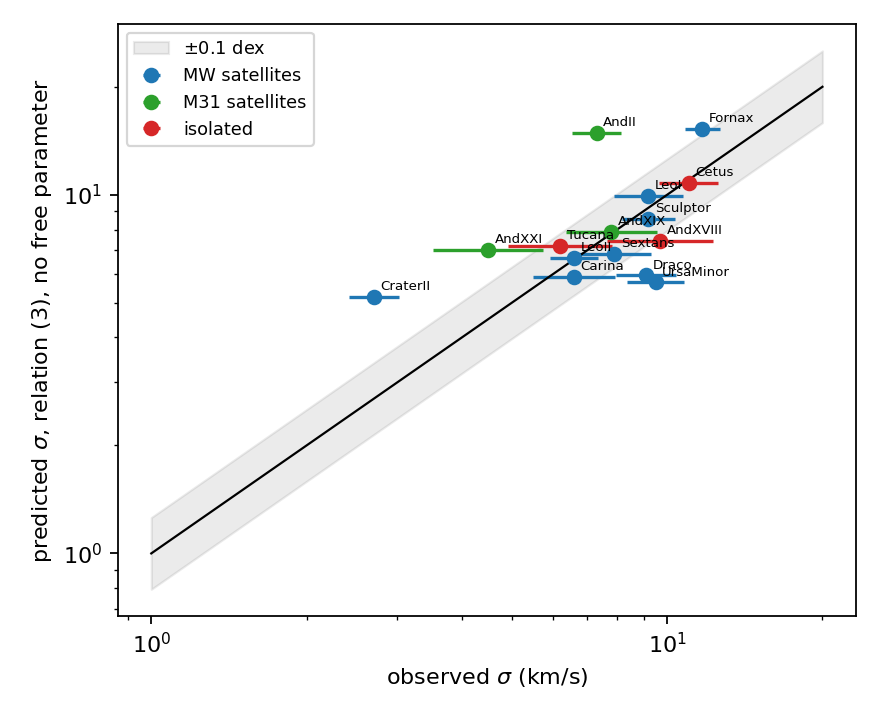
\includegraphics{figs_v2/fig6_dwarfs.png}
\caption{The dwarf protocol, first pass: predicted dispersion
from rule (3) with no per-object freedom against the observed value,
for Milky Way satellites, M31 satellites and isolated dwarfs; the band
is $\pm$ 0.1 dex. Nine of sixteen rows fall inside the per-object bar,
short of the pre-registered two-thirds; the residuals show no dependence
on the external field (three isolated objects).}
\end{figure}

\subsection{B.3 Halo models under the same evidence machinery}

Five halo and function models were scored against the relation under the nested-sampling treatment of Section 3.1, each pre-registered before its run, on the 147 SPARC galaxies of Section 3.2 with identical nuisance priors (disc and bulge mass-to-light ratios log-normal with 0.1 dex width about 0.5 and 0.7; distance and inclination Gaussian at SPARC's quoted errors), identical likelihood (velocity errors with an intrinsic scatter of 0.03 or 0.06 dex in $\log g$ added in quadrature; every model prefers 0.03) and identical sampler settings (dynesty, Speagle 2020, nested sampling after Skilling 2006; 300 live points); summed log-evidence differences are read on the usual scale (Trotta 2008) with the pre-registered threshold at 5. Models and their per-galaxy parameters: the relation at a universal $\rho_c=10^{7.45}$ (none); the relation with $\rho_c$ free (one, flat in $\log\rho_c$ over 6--10); the empirical acceleration relation (none); NFW (Navarro, Frenk \& White 1997) with $\log M_{200}$ flat over 8.5--14 and the concentration from Dutton \& Macci\`o (2014) with 0.11 dex scatter (two); NFW with the concentration flat over 0--2 dex (two); the DC14 profile of Di Cintio et al.~(2014), with inner slope, outer slope and transition set by the fitted stellar-to-halo mass ratio, clamped to its calibrated range, the same concentration prior and the DC14 concentration mapping (two); and a Burkert halo with flat priors on central density and core radius (two).

Table B.3. Summed log-evidence over 147 galaxies at 0.03 dex intrinsic scatter; maximum log-likelihood and distance shifts relative to the DC14 halo; median per-galaxy rms in $\log g$.

\begin{longtable}[]{@{}p{4.9cm}p{1.6cm}p{1.6cm}p{2.1cm}p{2.0cm}p{1.6cm}@{}}
\toprule
model & free per galaxy & $\sum\ln Z$ & $\Delta\sum\ln L_{\max}$ vs DC14 & galaxies with $|\Delta D|>2\sigma$ & rms (dex)\tabularnewline
\midrule
\endhead
this relation, $\rho_c$ free & 1 & $-9481$ & $+5$ & 12 & 0.033\tabularnewline
Burkert halo, core-surface-density prior & 2 & $-9484$ & $+90$ & 0 & 0.040\tabularnewline
DC14 halo, concentration prior & 2 & $-9545$ & 0 & 0 & 0.035\tabularnewline
Burkert halo, flat priors & 2 & $-9627$ & $+97$ & 1 & 0.032\tabularnewline
NFW, concentration free & 2 & $-9818$ & -- & 3 & 0.035\tabularnewline
NFW, concentration prior & 2 & $-9935$ & $-401$ & 4 & 0.035\tabularnewline
this relation, $\rho_c=10^{7.45}$ & 0 & $-10081$ & -- & 18 & 0.046\tabularnewline
acceleration relation & 0 & $-10191$ & -- & 15 & 0.044\tabularnewline
background normalisation (Appendix B.1) & 0 & $-10229$ & -- & 18 & 0.049\tabularnewline
\bottomrule
\end{longtable}

Three things follow. First, among models with per-galaxy freedom the ordering is the relation and the primed Burkert together, then DC14, the free Burkert, free NFW, NFW: every cored form beats NFW, and the relation's one parameter does what the feedback core's two do: the raw fit is equal and the evidence margin ($+65$) is the Occam cost of a second parameter the data constrain in one galaxy in ten (the posterior on the concentration offset is narrower than its 0.11 dex prior in 10\% of galaxies; the halo mass and the relation's $\rho_c$ are constrained in over 90\%). By effective count -- the sum of $1-(\sigma_{\rm post}/\sigma_{\rm prior})^2$ over a model's parameters -- the comparison is 0.9 against 1.3 parameters per galaxy (NFW 1.3, free NFW 1.6, primed Burkert 1.5, free Burkert 1.8). The free Burkert's deficit is the volume of its flat priors (five and three decades, both parameters constrained). A Burkert with the observed core-surface-density band as prior (Donato et al.~2009; $\log\mu_0$ Gaussian with 0.2 dex width about $\log 141$, core radius flat over $-1$ to 2 dex) is the fair cored comparator: it ties the relation in evidence ($-9484$ against $-9481$, within the sampling error of 3), with the same raw fit as the flat-prior Burkert ($+90$ over DC14) and no distance freedom; the relation's margin of 146 over the flat-prior Burkert was the volume of those priors. The tie is between one fitted parameter and two of which one is primed by an observed band: both are constrained, the core surface density to 0.12 dex within its 0.2 dex band and at the band's centre, the core radius to 0.1 dex, so by effective count the comparison is 0.9 against 1.5 parameters per galaxy; galaxy by galaxy the relation is ahead by 0.4 in the median, the Burkert winning the sum back in two galaxies {[}RESULT\_OCCAM\_20261101; PREREG\_BURKMU\_20261101; RESULT\_BURKMU\_20261102{]}. Second, among models with no per-galaxy freedom the relation at a universal density is best, ahead of the empirical function by 110 and of the background normalisation by 148; all three lose to every halo by hundreds, as any parameter-free law must against two numbers fitted to each curve. Third, the halo models use less distance freedom than the relation: DC14 moves no galaxy beyond two standard deviations, the relation with $\rho_c$ free moves twelve, the universal density eighteen. The per-galaxy audit is stable across the intrinsic-scatter settings: the relation loses to the haloes on NGC 247, F571-8, NGC 2403, UGC 12732 and UGC 128 and wins on IC 2574, NGC 3109, IC 4202 and ESO 563-G021. A quarter of the DC14 posteriors sit at the upper edge of the calibrated stellar-to-halo mass range, i.e.\ at halo masses an abundance-matching prior would forbid; imposing one would lower the halo's evidence and was not done. Pre-registrations, scripts and the per-galaxy evidence tables are in the repository (Data and code availability) {[}PREREG/RESULT\_CDM, CDM2, CDM3, RHOC\_BG{]}.

\section{Appendix C. Lensing: compatibility, truncation, satellites and the mass budget}\label{appendix-c.-lensing-compatibility-truncation-satellites-and-the-mass-budget}

The three purchases stated in the introduction rest on the following. Lensing: the nb mass lenses as ordinary non-relativistic mass (Section 1: its pressure and anisotropic stress are negligible), so the weak-lensing profile of an isolated galaxy is the dynamical one. Down to the truncation radius the tail is a singular isothermal sphere with $v^4=G a_0 M_b$, so lensing, dynamics and the MOND prediction coincide there; the truncation sits at $r_t=\sigma/\sqrt{2\pi G\rho_{\rm amb}}$: for the four stellar-mass bins of Mistele et al.~(2024b) ($\log M_*/M_\odot$ = 9.0--10.5, 10.5--10.8, 10.8--11.1, 11.1--11.5; $V_f$ = 141, 191, 214, 259 km/s) this is 3.2--5.9 Mpc at the closure value 35.5 and 0.8--1.4 Mpc at the 95\% bound 630 (for an $L^*$ galaxy, $M_b=3\times10^{10}$, 3.4 and 0.8 Mpc). $r_t$ is the matching radius of the isothermal tail; in the full solve with the subtraction the enclosed excess peaks about 20\% beyond it and the 10\% decline in $v_c$ sets in about 30\% inside it {[}RESULT\_N10 secs 2--3{]}; $r_t$ is used for scaling and the solve for the forecast (Figure 7).

On the baryonic-acceleration axis of the lensing relation this is $g_{\rm bar}(r_t)=GM_b/r_t^2\approx 4\times10^{-16}\,{\rm m\,s^{-2}}$ for an $L^*$ galaxy at the closure value ($6.5\times10^{-15}$ at the bound), at or just beyond the last bins of the stacks (Brouwer et al.~2021; Mistele et al.~2024b); the observed acceleration there is $g_{\rm obs}(r_t)=2\sigma\sqrt{2\pi G\rho_{\rm amb}}=2\sqrt{2\pi}\,(\sigma/c)\,a_0\approx 2\times10^{-13}\,{\rm m\,s^{-2}}$ at the closure value. MOND expects a decline at large radius too, from the external-field effect; Mistele et al.~(2024b, Discussion) write that it ``might become possible to perceive'' with better data, that it ``may be undetectable in the present data'', and that beyond 1 Mpc ``some mass bins possibly decline, but there is no clear departure from flatness''. The two expectations differ in kind -- an external-field decline is ordered by environment, the ambient truncation by $M_b^{1/4}$ at fixed $\rho_{\rm amb}$ (Section 6.3) -- but a quantitative comparison needs the orientation-averaged stacked profile in a non-uniform field, which we have not computed.

A fit of the truncated profile to their deprojected circular velocities (four mass bins, 41 points beyond 100 kpc, statistical and systematic errors in quadrature, $V_f$ free per bin) gives $\rho_{\rm amb}<630$ at 95\% ($\chi^2=21.5$ for 36 degrees of freedom). With the amplitude fixed by the relation rather than fitted ($V_f^4=Ga_0M_b$, also MOND's asymptote), the lensing flat speeds lie 5--13\% above the prediction at the stacked baryonic masses ($\chi^2=74$ for 41 points); a 0.1 dex increase in $M_b$, within the stellar-mass and gas systematics, gives $\chi^2=33$, and the ambient density is then bounded by 160--355 (95\%). The amplitude offset is shared with MOND and is not a discriminator. {[}pass10\_lensing\_fixedVf\_20261025.py; RESULT\_SIMROUND\_C1-C4 C4{]} Among the fits with $V_f$ free, a fit in the excess surface density gives $<630$ without a satellite term and $<1000$ with one. Restricted to 100 kpc--1 Mpc the data bound $\rho_{\rm amb}$ from above only ($<710$ at 95\%): they do not detect a truncation.

The mild preference for one over an untruncated tail ($\Delta\chi^2\approx6$) comes from the points beyond 1 Mpc, where isolation, the two-halo term and the deprojection's assumed continuation are least secure (the systematic column grows to 40--150 km/s there), so it is not a detection. The errors are treated as uncorrelated, and the systematic column (the uncertainty of their extrapolation beyond the last bin) is coherent across radius, so these numbers are indicative and the $\chi^2$ is too low; a forward model of $\Delta\Sigma$ with the KiDS covariance and a two-halo term is owed {[}RESULT\_LENSING\_FIT\_SATELLITES, erratum 2026-10-22: an earlier version of these fits misread two rows of the table{]}.

Under the source rule of Section 2.3 the satellites of an isolated galaxy are bodies with their own nb mass, each truncated by the host's tail; for a plausible ten satellites above $10^{8}$ $M_\odot$ within 1 Mpc they add \textasciitilde{}20--45\% to the host's enclosed nb mass at 1 Mpc (more for low-mass hosts) and little inside 0.5 Mpc, so the stacked profile beyond \textasciitilde{}0.5 Mpc is not the host's halo alone; the present data neither require nor exclude that term ($\Delta\chi^2\approx0.3$) {[}same file{]}.

Beyond $r_t$ the relation predicts a truncation of the excess mass whose radius scales as $M_b^{1/4}$ and $\rho_{\rm amb}^{-1/2}$, turning $\Delta\Sigma$ from $1/R$ toward $1/R^2$ between 1 and 5 Mpc (at the closure value, 0.95 of the untruncated value at 3 Mpc and 0.71 at 5), mass-ordered like the correlated-structure term, so separating the two needs mock stacks; that is a forecast for mass-binned stacks, not a present test. Early- and late-type lensing: Section 6.4. Mass budget. The closure value is taken as the global mean of all nb mass (Section 2.1), so the halos are drawn from the background and the budget closes by construction; the question is whether a non-negative background can supply them. Summed over the galaxy stellar mass function, isolated halos would carry a mean excess of $\sim$110 $M_\odot\,{\rm kpc}^{-3}$, 3.1 times the closure value: they cannot all exist. They need not: $r_t$ (3--6 Mpc) exceeds the typical separation of galaxies (a few Mpc), so a tail is cut by its neighbours' before it reaches the background, and isolated-halo sums overcount the same mass.

A mean-field estimate with the observed galaxy clustering (Zehavi et al.~2011), in which each tail ends where it meets the mean nb density around its galaxy, brings the halo excess to 0.4 of the closure value and leaves a background of 0.5--0.7 of it between galaxies, while isolated galaxies keep truncation radii of 2.7--5.2 Mpc. The estimate is biased low: it places every galaxy at the mean density around it, and for dwarfs that mean is set by the few that sit inside a host; if galaxies below $M_*\sim10^{9.5}\,M_\odot$ are instead left untruncated, the background reaches zero. The budget is therefore open, with a mean-field indication that it can close; a calculation over the distribution of local densities, satellites included, is owed (Section 7). {[}RESULT\_N11\_PASS1\_20261026; PREREG\_N11\_20261026{]} No suppressing external-field effect: the internal dynamics of a bound system depend on their surroundings only through the small enhancing ambient and nesting terms (Section 2.3), because the response is to the body's own potential; MOND's external-field effect acts at first order, and the difference is the discriminator of Section 4.4 and 6.2. History-blindness: identical present baryons in the same local background give identical nb mass. This predicts no dependence of present structure on its past and no dark sub-haloes without galaxies; it is untested here and is listed as a prediction. The baryons come first: a cloud that becomes self-gravitating acquires its nb mass on its own dynamical time, not after a halo has formed.

\begin{figure}
\centering
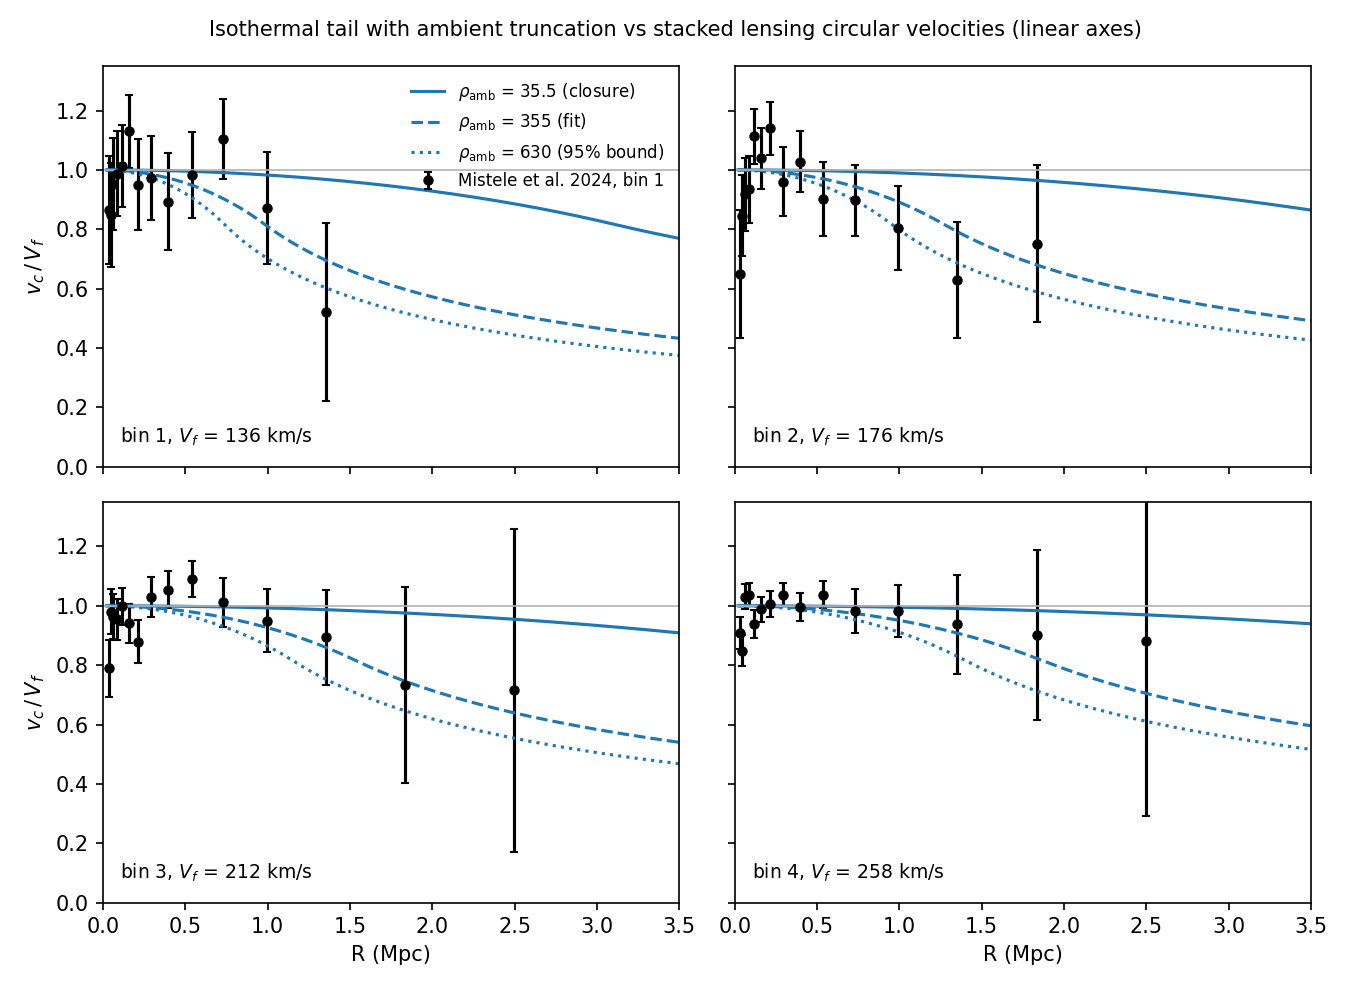
\includegraphics[width=\textwidth]{figs_v2/fig7_truncation.png}
\caption{The ambient truncation against the stacked weak-lensing circular velocities of Mistele et al.~(2024b), Table 1, four stellar-mass bins, on linear axes. Points: their deprojected $v_c$ with statistical and systematic errors in quadrature, normalised by the bin's flat speed $V_f$ fitted at $\rho_{\rm amb}=35.5$ (which favours the closure curve visually). Curves: the isothermal tail with the ambient term subtracted and cut at $r_t=\sigma/\sqrt{2\pi G\rho_{\rm amb}}$, for $\rho_{\rm amb}=35.5$ (closure), 355 (the value the points beyond 1 Mpc would prefer, shown for reference and not adopted) and 630 (95\% bound) $M_\odot\,{\rm kpc}^{-3}$. The decline begins before $r_t$ because the subtracted ambient term already lowers the enclosed excess; beyond $r_t$ the excess mass is constant and $v_c$ falls as $r^{-1/2}$. The most massive bin truncates last ($r_t\propto M_b^{1/4}$) and is the flattest. [fig7\_truncation\_20261021.py; RESULT\_LENSING\_FIT\_SATELLITES]}
\end{figure}


\section{Appendix D. The environment test in full}\label{appendix-d.-the-environment-test-in-full}

Chae et al.~(2020, 2021) fit each SPARC curve with an external-field parameter $\tilde e$, marginalising mass-to-light ratios, distance and inclination, on a sample selected to be unbiased with respect to outer decline, and detect $\tilde e>0$ on the sample median ($4.4\sigma$; 97 of 143 positive) with a contrast between underdense and overdense regions of the cosmic web; they also report that the galaxy-by-galaxy correlation of $\tilde e$ with the environmental field is not recoverable at current errors (their sec 4.2). Our test is weaker than theirs: the low-acceleration residual from the acceleration relation, at fixed mass-to-light ratio, distance and inclination, over points with $g_{\rm bar}$ \textless{} $a_0$/3 (a selection their Appendix B notes favours less-declining curves), regressed on their environmental field. It gives -0.12 $\pm$ 0.16 dex per dex at fixed mass and surface density. The external-field effect, evaluated galaxy by galaxy with Chae et al.'s own formula at their field values, predicts -0.08 for this sample; the relation predicts 0. The sample does not separate the two; the point estimate lies at the external-field value. The outer-slope statistic is null (-0.03 $\pm$ 0.21).

Chae et al.~(2020) report a detection with the external-field sign from per-galaxy fits; Paranjape \& Sheth (2022) argue its significance is compromised by rotation-curve uncertainties and the simulation-based field estimates, and that a qualitatively similar signal is expected in LCDM from clustering-property correlations. We then applied their statistic itself: their MOND-plus-external-field model fitted to each curve with mass-to-light ratios, distance and inclination marginalised under the SPARC priors, on their $x_{0,3}$ selection (102 galaxies).

On the observed curves this reproduces their per-galaxy values (rank correlation 0.88) and a positive median, +0.016 (their tabulated fits: +0.025, 61\% positive). Fitted to the relation's own curves, which contain no external field, the same model returns a positive median too: +0.012 (57\% positive) at the single density $10^{7.45}$, and +0.022 (60\%) at the fitted densities. The cored-isothermal outer shape is read by their model as an external field of about half the size they detect; the median-$\tilde e$ detection therefore does not by itself discriminate suppression from this relation.

What would is the dependence of $\tilde e$ on the environmental field; on this subsample it is weak and not of the external-field sign (rank correlation -0.26 for 60 galaxies with field values; -0.10 for their tabulated values), consistent with their own statement that the galaxy-by-galaxy correlation is not recoverable at current errors. Splitting the 60 galaxies with field values into terciles, $\tilde e$ is higher in the LOW-field tercile for the observed curves (+0.05 against 0.00, p = 0.03) and for their own fits (+0.09 against +0.03), and the relation's curves show the same contrast (p = 0.02); the observed-minus-model difference has no field dependence (p = 0.76). The regional contrast they report (underdense against overdense regions of the cosmic web) uses region assignments not available to us and is the remaining discriminator, untested here. This is the note's open weak point. {[}RESULT\_N8B + addendum; RESULT\_N8D{]}

\section{Appendix E. Cloud-9, lensing by morphology, pairwise forces}\label{appendix-e.-cloud-9-lensing-by-morphology-pairwise-forces}

\subsection{E.1 Cloud-9}

The starless HI cloud near M94 ($M_{\rm HI}\sim10^6\,M_\odot$, $r\sim1.4$ kpc, $W_{50}=12$ km/s, non-rotating,
$D\sim4.4$ Mpc, no stars above $10^{3.5}$ $M_\odot$;
Benitez-Llambay et al.~2024, arXiv:2406.18643; Anand et al.~2025,
arXiv:2508.20157{[}; LIT\_CLOUD9\_RELHIC\_20261018{]}) has a random
speed (\textasciitilde{}5 km/s) above its self-gravity speed
(\textasciitilde{}1.8 km/s) and a Jeans length (\textasciitilde{}8 kpc)
larger than itself, so its gas alone does not bind it. Under the source rule of
Section 2.3 it nonetheless carries nb mass, set by its $\rho_c$: for
$\log\rho_c\lesssim5.5$ too little to bind it (it is then confined by its
surroundings or dispersing), for $\log\rho_c\gtrsim6$ enough
($1$--$7\times10^7\,M_\odot$ inside 1.4 kpc, of the order of the dynamical mass
$\sim2.5\times10^7\,M_\odot$ its line width implies)
{[}RESULT\_BODY\_RULE\_20261022{]}. LCDM (RELHIC) places it in a
$\sim5\times10^9\,M_\odot$ halo; MOND gives a modest external-field boost.
One object, three different answers. {[}BALLOT CLOUD9-1 2026-10-18
12:00; CLOUD9-DFX 2026-10-19 18:10; inputs from LIT\_CLOUD9\_RELHIC{]}

\subsection{E.2 Lensing by morphology}

Early- and late-type lensing relations are identical at fixed baryonic mass under the dynamical assumption of Section 2.2, whereas a conserved completion predicts an early-type excess growing with merger history (about 0.04--0.075 dex in $g_{\rm obs}$ per merger); the data show a $\ge6\sigma$ difference in Brouwer et al.~(2021) and none significant after the stellar-mass, hot-gas and isolation corrections of Mistele et al.~(2024a,b), who recover Brouwer's difference with Brouwer's choices (Appendix C and the merger estimate of Section 7). Pairwise forces at 30-230 Mpc.

\subsection{E.3 Pairwise forces}

Gallardo et al.~(2026) find an inverse-square pairwise force law from the kinetic Sunyaev-Zel'dovich effect: the acceleration between halo pairs scales as $r^{-n}$ with $n=2.1\pm0.3$ at 30--230 Mpc (ACT with SDSS). Any real-mass theory passes this
in shape by construction; the amplitude requires the Mpc-scale nb budget
and is open. The external field invoked to recover inverse-square behaviour in MOND (a few per cent of $a_0$) is at the upper end of, or above, the values Chae et al.~(2021) assign to SPARC galaxies (0.002--0.018 $a_0$) and the few-per-cent estimate for the field of large-scale structure (Famaey \& McGaugh 2012, Section 6.3; McGaugh 2026a gives 1--2\%).

\section{Appendix F. Relation to v1.0.14}\label{appendix-f.-relation-to-v1.0.14}

The v1.0.14 preprint derived its augmented Poisson equation with the wrong operator sign ($-k^2$; the bump substitution gives $+k^2$; erratum posted 2026-10), withdrew its Yukawa exterior and $\nu$-function with it, and argued the uniqueness of a linear law (Appendix F) that the present nonlinear relation supersedes. Its account of the Bullet cluster (p.\textasciitilde{}25, Fig. 6), that lensing responds to the gradient of surface density, is withdrawn: convergence is surface density, and the Clowe et al.~(2006) apertures show baryons at the plasma peaks equal to or above those at the galaxies. A post-v1.0.14 working wide-binary number, $\gamma$ = 1.13-1.26 (2026-10-15), came from a floor-clipped phantom-density construction under an intermediate law and is superseded by the Newtonian prediction of Section 6.1. Its three-regime picture (Newtonian, MOND-like, and an exponential falloff beyond) and its claim that the Gaia DR3 decline of the Milky Way curve is a regime MOND cannot predict are withdrawn: the Yukawa cutoff at $k^{-1}\approx14$ kpc that defined the outer regime went with the operator sign, and the MOND comparison (rising to \textasciitilde{}204 km/s at 27 kpc) normalised MOND at 10 kpc rather than computing it from the baryons. Computed from the same baryons, MOND and the present relation both decline across that range (Section 3.2, Appendix A); the decline is the transition, and the relation's departure from MOND phenomenology lies at the ambient truncation, at 0.8--3.4 Mpc (Section 6.3). v2.0.1 revises v2.0.0 under the same concept DOI.

\section{Appendix G. A numerical correspondence}\label{appendix-g}

We record a numerical correspondence without drawing a cosmological
conclusion from it. The global mean of the ambient density is taken at
$a_0^2/Gc^2=35.5\,M_\odot\,{\rm kpc}^{-3}$ (Section 2.1). The Planck
physical densities, which do not depend on the Hubble constant, are
$\Omega_ch^2=0.120$ for non-baryonic matter and $\Omega_bh^2=0.0224$ for
baryons, i.e.\ 33.3 and 6.2 $M_\odot\,{\rm kpc}^{-3}$ today (Planck
Collaboration 2020). The closure value is 1.06 times the first; added to
the baryons it is 1.05 times the total matter density. Three cautions keep
this a correspondence and not a result:
\begin{itemize}
\item[(i)] $a_0$ is known to about 20\% (systematic; McGaugh, Lelli \& Schombert 2016), so the closure density is uncertain by about 40\%; agreement at the 5\% level is better than the inputs justify.
\item[(ii)] The closure carries an undetermined factor of order unity (a uniform sphere cut off at the causal length gives $2\pi$ rather than 1), so the match depends on a choice we have not derived.
\item[(iii)] Whether the nb mass of this note is the non-baryonic matter of cosmology is not addressed here (Section 1).
\end{itemize}
We note it because the relation's one cosmological input, set by an acceleration measured in galaxies, lands on the measured non-baryonic density, and because the same $a_0$ fixes where the baryon term saturates (Section 2.1).

The correspondence has a reading within the relation, which we state as a reading and not a derivation. In MOND $a_0$ is a constant of the interpolating function, and its closeness to $cH_0$ (Milgrom 1983) or to $c^2\sqrt{\Lambda}$ (Milgrom 1999) is noted but unexplained within the theory. Here the background potential, $\Phi_{\rm bg}\sim c^2$ over a horizon length $L\sim c/\sqrt{G\bar\rho}$ (Section 2.1), has the gradient scale $c\sqrt{G\bar\rho}$, which is $a_0$ to within the factor of order unity of caution (ii); with the Planck matter density the statement reads $a_0=c\sqrt{G\rho_m}$ to 6 per cent, independent of $H_0$. The same background is the ambient density that ends every halo (Section 2.2). One posited quantity thus plays three roles that are three separate facts in MOND: the acceleration scale, the halo edge, and the cosmic-density coincidence. On this reading the background is the response of the nb component to the baryons of the universe as a whole, with the velocity parameter of that outermost system, $c$, so that distant baryons set the background and not the bump: a galaxy's potential perturbs the background by $\varphi/c^2\sim10^{-7}$, while the galaxy's own halo responds with its own $\sigma$ (Section 2.3). What is open is what makes this a reading: the factor of order unity, the horizon profile that would fix it, and the ratio of $4\times10^6$ between $c^2$ and a galaxy's $\sigma^2$ {[}NOTE\_A0\_CLOSURE\_20260930 secs 10-11, 14{]}.

\section{Appendix H. No action in the canonical class}\label{appendix-h}

We show why eqs.~(1)--(2) cannot come from an action with two canonical scalar fields and local couplings. Let $\psi$ be the baryons' potential and $\chi$ the nb mass's own potential, with matter coupled to $\Phi=\psi+\chi$, and take the most general such Lagrangian with constant kinetic coefficients and a local potential $R$:
\[
\mathcal{L}=-\frac{1}{8\pi G}\left(a|\nabla\psi|^2+2b\,\nabla\psi\cdot\nabla\chi+c|\nabla\chi|^2\right)-\rho_b(\psi+\chi)-R(\psi,\chi).
\]
The field equations are $(a\nabla^2\psi+b\nabla^2\chi)/4\pi G=\rho_b+R_\psi$ and $(b\nabla^2\psi+c\nabla^2\chi)/4\pi G=\rho_b+R_\chi$. We require $\nabla^2\psi=4\pi G\rho_b$ and $\nabla^2\chi=4\pi G\rho_{\rm nb}$ for any baryon distribution. Because $R$ depends on the fields and not on $\rho_b$, the coefficients of $\rho_b$ must cancel, which fixes $a=b=1$; then $R_\psi=\rho_{\rm nb}$ and $R_\chi=c\,\rho_{\rm nb}$. A function $R$ with these derivatives exists only if $\partial R_\psi/\partial\chi=\partial R_\chi/\partial\psi$, that is
\[
\frac{\partial\rho_{\rm nb}/\partial\chi}{\partial\rho_{\rm nb}/\partial\psi}=c,
\]
a constant: $\rho_{\rm nb}$ must depend on the single combination $\psi+c\,\chi$.

In eq.~(1) the nb mass responds to its own potential with slope $1/\sigma^2$ and to the baryons' with slope $S'(x_b)/\sigma^2$, so the ratio above is $1/S'(x_b)=\cosh^2(x_b/2)$ for $S=2\tanh(x/2)$. It is constant only if $S$ is linear, that is, without the saturation. The ratio is also fixed to 1 by the tail, which needs the nb mass to respond to its own potential with the same $\sigma$; then $c=1$, the kinetic matrix becomes degenerate, and the two fields combine into $\Phi$ alone: the single-field action of a perfect fluid, $\mathcal{L}=-|\nabla\Phi|^2/8\pi G-\rho_b\Phi-R(\Phi)$, whose response saturates on the total potential. That removes the tail. An isothermal sphere's own potential below its edge is $\sim2\sigma^2\ln(r_t/r)$, so the response saturates throughout $r<r_t/e$, the nb density stays near $\rho_c$, and the enclosed mass grows as $r^3$.

Numerically, the Milky Way curve then has an rms of 212 km/s at the universal $\rho_c$ and 40 km/s at the best $\rho_c$, against 19.7 and 8.6 for eqs.~(1)--(2). Saturation on the baryons together with an isothermal self-tail is therefore not variational in this class. Gradient couplings of the AQUAL type lie outside it; the simplest of them, a saturation through $|\nabla\psi|$, makes the gravitating nb density a total divergence with zero net mass, and the class is otherwise untested. {[}lagrangian\_checks\_20261021.py; lawA\_total\_potential\_20261021.py; DERIVATION\_ACTION\_20261021{]}

\section{Data and code availability}\label{data-code}

The rotation curves and baryon models are from SPARC (Lelli, McGaugh \& Schombert 2016a). The source of this note, the analysis scripts and their outputs, and the pre-registrations of the tests are at \url{https://github.com/Jimmnj/gprf-v2}, archived as doi:10.5281/zenodo.23995058 (all versions: doi:10.5281/zenodo.23781855); a script there downloads SPARC and checks it against the copies used. Each pre-registration file is dated in its header and was written before its run; the repository is committed periodically, so its history bounds rather than timestamps each one, and the Zenodo archive freezes the set.

\section{Funding and conflicts of interest}

No funding was received for this work. The author declares no conflicts of interest.

\section{AI usage}\label{ai-usage}

This work was carried out with extensive assistance from Anthropic's
Claude models: literature search and verification of references, code
for the solvers and fits, numerical runs, drafting and editing of text,
and simulated referee reports used as stress tests. The author set the
questions and the hypotheses, pre-registered the tests, decided every
result's status and every claim's wording, and takes full responsibility
for the content.

\section{References}\label{references}

{\small
\begin{list}{}{\setlength{\leftmargin}{1.5em}\setlength{\itemindent}{-1.5em}\setlength{\itemsep}{1pt}\setlength{\parsep}{0pt}}
\item Anand, G. S., Ben\'{\i}tez-Llambay, A., Beaton, R., et al.\ 2025, ApJL 993, L55 (arXiv:2508.20157)
\item Angus, G. W.\ 2009, MNRAS 394, 527 (arXiv:0805.4014)
\item Angus, G. W., Gentile, G., Swaters, R., et al.\ 2015, MNRAS 451, 3551 (arXiv:1505.05522)
\item Aniyan, S., Freeman, K. C., Gerhard, O. E., Arnaboldi, M., \& Flynn, C.\ 2016, MNRAS 456, 1484 (arXiv:1511.06781)
\item Banik, I., et al.\ 2024, MNRAS 527, 4573 (arXiv:2311.03436)
\item Bekenstein, J., \& Milgrom, M.\ 1984, ApJ 286, 7
\item Bershady, M. A., Verheijen, M. A. W., Swaters, R. A., et al.\ 2010, ApJ 716, 198 (arXiv:1004.4816)
\item Ben\'{\i}tez-Llambay, A., Dutta, R., Fumagalli, M., et al.\ 2024, ApJ 973, 61 (arXiv:2406.18643)
\item Berezhiani, L., \& Khoury, J.\ 2015, PRD 92, 103510 (arXiv:1507.01019)
\item Blanchet, L.\ 2007, CQG 24, 3529 (arXiv:astro-ph/0605637)
\item Blanchet, L., \& Le Tiec, A.\ 2008, PRD 78, 024031 (arXiv:0804.3518)
\item Borukhovetskaya, A., et al.\ 2022, MNRAS 512, 5247 (arXiv:2112.01540)
\item Brans, C., \& Dicke, R. H.\ 1961, Phys.\ Rev.\ 124, 925
\item Brouwer, M. M., et al.\ 2021, A\&A 650, A113 (arXiv:2106.11677)
\item Bruneton, J.-P., Liberati, S., Sindoni, L., \& Famaey, B.\ 2009, JCAP 03, 021 (arXiv:0811.3143)
\item Burkert, A.\ 1995, ApJL 447, L25 (arXiv:astro-ph/9504041)
\item Caldwell, N., et al.\ 2017, ApJ 839, 20 (arXiv:1612.06398)
\item Chae, K.-H.\ 2023, ApJ 952, 128 (arXiv:2305.04613)
\item Chae, K.-H.\ 2024a, ApJ 960, 114; erratum doi:10.3847/1538-4357/ad40ac (arXiv:2309.10404)
\item Chae, K.-H.\ 2024b, ApJ 972, 186 (arXiv:2402.05720)
\item Chae, K.-H.\ 2025, ApJ 985, 210 (arXiv:2502.09373)
\item Chae, K.-H., et al.\ 2020, ApJ 904, 51
\item Chae, K.-H., et al.\ 2021, ApJ 921, 104 (arXiv:2109.04745)
\item Chae, K.-H., Lee, B.-C., Hernandez, X., et al.\ 2026, arXiv:2601.21728 (submitted)
\item Chae, K.-H., \& Yoon, Y.\ 2026, arXiv:2607.14450
\item Chandra, V., Naidu, R. P., Conroy, C., et al.\ 2025, ApJ 988, 156 (arXiv:2406.01676)
\item Clowe, D., et al.\ 2006, ApJL 648, L109 (arXiv:astro-ph/0608407)
\item Collins, M. L. M., et al.\ 2020, MNRAS 491, 3496 (arXiv:1910.12879)
\item Cookson, S. A., Banik, I., El-Badry, K., et al.\ 2026, MNRAS, doi:10.1093/mnras/stag342 (arXiv:2602.24035)
\item Danieli, S., et al.\ 2019, ApJL 874, L12 (arXiv:1901.03711)
\item Debattista, V. P., \& Sellwood, J. A.\ 2000, ApJ 543, 704 (arXiv:astro-ph/0006275)
\item Desmond, H.\ 2023, MNRAS 526, 3342 (arXiv:2303.11314)
\item Di Cintio, A., Brook, C. B., Dutton, A. A., et al.\ 2014, MNRAS 441, 2986 (arXiv:1404.5959)
\item Donato, F., et al.\ 2009, MNRAS 397, 1169 (arXiv:0904.4054)
\item Dutton, A. A., \& Macci\`o, A. V.\ 2014, MNRAS 441, 3359 (arXiv:1402.7073)
\item Erkal, D., et al.\ 2019, MNRAS 487, 2685 (arXiv:1812.08192)
\item Koposov, S. E., Erkal, D., Li, T. S., et al.\ 2023, MNRAS 521, 4936 (arXiv:2211.04495)
\item Gentile, G., Famaey, B., Zhao, H., \& Salucci, P.\ 2009, Nature 461, 627 (arXiv:0909.5203)
\item Famaey, B., Khoury, J., \& Penco, R.\ 2018, JCAP 03, 038 (arXiv:1712.01316)
\item Famaey, B., \& McGaugh, S. S.\ 2012, Living Rev.\ Relativ.\ 15, 10 (arXiv:1112.3960)
\item Famaey, B., McGaugh, S., \& Milgrom, M.\ 2018, MNRAS 480, 473 (arXiv:1804.04167)
\item Felten, J. E.\ 1984, ApJ 286, 3
\item Fragkoudi, F., et al.\ 2021, A\&A 650, L16 (arXiv:2011.13942)
\item Gallardo, P. A., et al.\ 2026, PRL 136, 151002 (doi:10.1103/rk8v-rcm3)
\item Haghi, H., et al.\ 2019, MNRAS 487, 2441 (arXiv:1906.03268)
\item Harvey, D., et al.\ 2015, Science 347, 1462 (arXiv:1503.07675)
\item Hernandez, X., Chae, K.-H., \& Aguayo-Ortiz, A.\ 2024, MNRAS 533, 729 (arXiv:2312.03162)
\item Hossenfelder, S.\ 2017, PRD 95, 124018 (arXiv:1703.01415)
\item Ianjamasimanana, R., et al.\ 2015, AJ 150, 47 (doi:10.1088/0004-6256/150/2/47)
\item Iorio, G., Fraternali, F., Nipoti, C., et al.\ 2017, MNRAS 466, 4159 (arXiv:1611.03865)
\item Ji, A. P., et al.\ 2021, ApJ 921, 32 (arXiv:2106.12656)
\item Jiao, Y., et al.\ 2023, A\&A 678, A208 (arXiv:2309.00048)
\item Kaplinghat, M., Ren, T., \& Yu, H.-B.\ 2020, JCAP 06, 027 (arXiv:1911.00544)
\item Kaplinghat, M., Tulin, S., \& Yu, H.-B.\ 2016, PRL 116, 041302 (arXiv:1508.03339)
\item Khoury, J.\ 2015, PRD 91, 024022 (arXiv:1409.0012)
\item King, I. R.\ 1966, AJ 71, 64
\item Kormendy, J., \& Freeman, K. C.\ 2016, ApJ 817, 84 (arXiv:1411.2170)
\item Lelli, F., McGaugh, S. S., \& Schombert, J. M.\ 2016a, AJ 152, 157 (arXiv:1606.09251)
\item Lelli, F., McGaugh, S. S., \& Schombert, J. M.\ 2016b, ApJL 816, L14 (arXiv:1512.04543)
\item Lelli, F., McGaugh, S. S., Schombert, J. M., \& Pawlowski, M. S.\ 2016c, ApJL 827, L19 (arXiv:1607.02145)
\item Lelli, F., et al.\ 2017, ApJ 836, 152 (arXiv:1610.08981)
\item Lelli, F., McGaugh, S. S., Schombert, J. M., Desmond, H., \& Katz, H.\ 2019, MNRAS 484, 3267 (arXiv:1901.05966)
\item Lelli, F., Marasco, A., Davis, T. A., et al.\ 2026, in Advancing Astrophysics with the SKA II (arXiv:2608.07290)
\item Leroy, A. K., Walter, F., Bigiel, F., et al.\ 2009, AJ 137, 4670 (arXiv:0905.4742)
\item Li, P., et al.\ 2018, A\&A 615, A3 (arXiv:1803.00022)
\item Li, P., Lelli, F., McGaugh, S., \& Schombert, J.\ 2020, ApJS 247, 31 (arXiv:2001.10538)
\item LZ Collaboration 2025, PRL 135, 011802 (arXiv:2410.17036)
\item Martinsson, T. P. K., Verheijen, M. A. W., Westfall, K. B., et al.\ 2013a, A\&A 557, A130 (arXiv:1307.8130)
\item Martinsson, T. P. K., Verheijen, M. A. W., Westfall, K. B., et al.\ 2013b, A\&A 557, A131 (arXiv:1308.0336)
\item Marsen, J. R.\ 2026, GPRF Paper I, v1.0.14, Zenodo, doi:10.5281/zenodo.20943223
\item McGaugh, S. S.\ 2016, ApJL 832, L8 (arXiv:1610.06189)
\item McGaugh, S. S.\ 2019, ApJ 885, 87 (arXiv:1909.11158)
\item McGaugh, S. S.\ 2015, Can. J. Phys. 93, 250 (arXiv:1404.7525)
\item McGaugh, S. S.\ 2023, `Required dark matter properties', Triton Station (blog), 17 Aug 2023
\item McGaugh, S. S.\ 2026a, `The External Field Effect and Tests of MOND on Cosmological Scales', Triton Station (blog), 27 Aug 2026, doi:10.59350/57294-avw93
\item McGaugh, S. S.\ 2026b, `Why the search for particle dark matter is hopeless, part 1', Triton Station (blog), 26 Oct 2026, https://tritonstation.com/2026/10/26/why-the-search-for-particle-dark-matter-is-hopeless-part-1/
\item McGaugh, S. S., \& Milgrom, M.\ 2013a, ApJ 766, 22 (arXiv:1301.0822)
\item McGaugh, S. S., \& Milgrom, M.\ 2013b, ApJ 775, 139 (arXiv:1308.5894)
\item McGaugh, S. S., Lelli, F., \& Schombert, J. M.\ 2016, PRL 117, 201101 (arXiv:1609.05917)
\item McGaugh, S. S., Lelli, F., Li, P., \& Schombert, J. M.\ 2019, in IAU Symp.~353, Galactic Dynamics in the Era of Large Surveys (arXiv:1909.02011)
\item Milgrom, M.\ 1983, ApJ 270, 365
\item Milgrom, M.\ 1986, ApJ 306, 9
\item Milgrom, M.\ 1999, Phys. Lett. A 253, 273 (arXiv:astro-ph/9805346)
\item Milgrom, M.\ 2009, MNRAS 398, 1023 (arXiv:0909.5184)
\item Milgrom, M.\ 2016, PRL 117, 141101 (arXiv:1607.05103)
\item Milgrom, M.\ 2010, MNRAS 403, 886 (arXiv:0911.5464)
\item Mistele, T., McGaugh, S., \& Hossenfelder, S.\ 2023a, JCAP 09, 004 (arXiv:2303.08560)
\item Mistele, T., McGaugh, S., \& Hossenfelder, S.\ 2023b, A\&A 676, A100 (arXiv:2301.03499)
\item Mistele, T., et al.\ 2024a, JCAP 04, 020 (arXiv:2310.15248)
\item Mistele, T., et al.\ 2024b, ApJL 969, L3 (arXiv:2406.09685)
\item Navarro, J. F., Frenk, C. S., \& White, S. D. M.\ 1997, ApJ 490, 493 (arXiv:astro-ph/9611107)
\item Oman, K. A., et al.\ 2015, MNRAS 452, 3650 (arXiv:1504.01437)
\item Ou, X., et al.\ 2024, MNRAS 528, 693 (arXiv:2303.12838)
\item PandaX-4T Collaboration 2025, PRL 134, 011805 (arXiv:2408.00664)
\item Paranjape, A., \& Sheth, R. K.\ 2022, MNRAS 517, 130 (arXiv:2112.00026)
\item Pflamm-Altenburg, J.\ 2025, A\&A 703, A68
\item Pittordis, C., et al.\ 2025, Open J.\ Astrophys., doi:10.33232/001c.142887 (arXiv:2504.07569)
\item Planck Collaboration 2020, A\&A 641, A6 (arXiv:1807.06209)
\item Ren, T., Kwa, A., Kaplinghat, M., \& Yu, H.-B.\ 2019, PRX 9, 031020 (arXiv:1808.05695)
\item Roshan, M., et al.\ 2021, MNRAS 508, 926 (arXiv:2106.10304)
\item Salucci, P., \& Burkert, A.\ 2000, ApJL 537, L9 (arXiv:astro-ph/0004397)
\item Sancisi, R.\ 2004, IAU Symp.\ 220, 233 (arXiv:astro-ph/0311348)
\item Sanders, J. L., Evans, N. W., \& Dehnen, W.\ 2018, MNRAS 478, 3879 (arXiv:1802.09537)
\item Schombert, J., McGaugh, S., \& Lelli, F.\ 2019, MNRAS 483, 1496 (arXiv:1811.10579)
\item Sciama, D. W.\ 1953, MNRAS 113, 34
\item Shen, Z., et al.\ 2021, ApJL 914, L12 (arXiv:2104.03319)
\item Shen, Z., et al.\ 2023, ApJ 957, 6 (arXiv:2309.08592)
\item Shipp, N., Erkal, D., Drlica-Wagner, A., et al.\ 2021, ApJ 923, 149 (arXiv:2107.13004)
\item Skilling, J.\ 2006, Bayesian Analysis 1, 833
\item Skordis, C., \& Zlosnik, T.\ 2021, PRL 127, 161302 (arXiv:2007.00082)
\item Speagle, J. S.\ 2020, MNRAS 493, 3132 (arXiv:1904.02180)
\item Spergel, D. N., \& Steinhardt, P. J.\ 2000, PRL 84, 3760 (arXiv:astro-ph/9909386)
\item Toomre, A.\ 1963, ApJ 138, 385
\item Trotta, R.\ 2008, Contemp.\ Phys.\ 49, 71 (arXiv:0803.4089)
\item Tulin, S., \& Yu, H.-B.\ 2018, Phys.\ Rep.\ 730, 1 (arXiv:1705.02358)
\item van Dokkum, P., et al.\ 2018, Nature 555, 629 (arXiv:1803.10237)
\item van Dokkum, P., Danieli, S., Abraham, R., et al.\ 2019, ApJL 874, L5 (arXiv:1901.05973)
\item Vasiliev, E., Belokurov, V., \& Erkal, D.\ 2021, MNRAS 501, 2279 (arXiv:2009.10726)
\item Vivas, A. K., Walker, A., Mart\'{\i}nez-V\'azquez, C., et al.\ 2026, AJ 171, 84 (arXiv:2512.05535)
\item Walker, M. G., et al.\ 2009, ApJ 704, 1274; erratum 2010, ApJ 710, 886 (arXiv:0906.0341)
\item XENONnT Collaboration 2025, PRL 135, 221003 (doi:10.1103/msw4-t342)
\item Zehavi, I., et al.\ 2011, ApJ 736, 59 (arXiv:1005.2413)
\end{list}}

\end{document}
